%% bare_conf_compsoc.tex
%% V1.4a
%% 2014/09/17
%% by Michael Shell
%% See:
%% http://www.michaelshell.org/
%% for current contact information.
%%
%% This is a skeleton file demonstrating the use of IEEEtran.cls
%% (requires IEEEtran.cls version 1.8s or later) with an IEEE Computer
%% Society conference paper.
%%
%% Support sites:
%% http://www.michaelshell.org/tex/ieeetran/
%% http://www.ctan.org/tex-archive/macros/latex/contrib/IEEEtran/
%% and
%% http://www.ieee.org/

%%*************************************************************************
%% Legal Notice:
%% This code is offered as-is without any warranty either expressed or
%% implied; without even the implied warranty of MERCHANTABILITY or
%% FITNESS FOR A PARTICULAR PURPOSE! 
%% User assumes all risk.
%% In no event shall IEEE or any contributor to this code be liable for
%% any damages or losses, including, but not limited to, incidental,
%% consequential, or any other damages, resulting from the use or misuse
%% of any information contained here.
%%
%% All comments are the opinions of their respective authors and are not
%% necessarily endorsed by the IEEE.
%%
%% This work is distributed under the LaTeX Project Public License (LPPL)
%% ( http://www.latex-project.org/ ) version 1.3, and may be freely used,
%% distributed and modified. A copy of the LPPL, version 1.3, is included
%% in the base LaTeX documentation of all distributions of LaTeX released
%% 2003/12/01 or later.
%% Retain all contribution notices and credits.
%% ** Modified files should be clearly indicated as such, including  **
%% ** renaming them and changing author support contact information. **
%%
%% File list of work: IEEEtran.cls, IEEEtran_HOWTO.pdf, bare_adv.tex,
%%                    bare_conf.tex, bare_jrnl.tex, bare_conf_compsoc.tex,
%%                    bare_jrnl_compsoc.tex, bare_jrnl_transmag.tex
%%*************************************************************************


% *** Authors should verify (and, if needed, correct) their LaTeX system  ***
% *** with the testflow diagnostic prior to trusting their LaTeX platform ***
% *** with production work. IEEE's font choices and paper sizes can       ***
% *** trigger bugs that do not appear when using other class files.       ***                          ***
% The testflow support page is at:
% http://www.michaelshell.org/tex/testflow/

\documentclass[conference,compsoc]{IEEEtran}
%%============================================%%
\usepackage{amsmath}
\usepackage{graphicx}
\usepackage{algorithm2e}
\usepackage{color}
\usepackage{url}
\usepackage{makecell}
\usepackage{epstopdf}
\usepackage{comment}
%%============================================%%
% Some/most Computer Society conferences require the compsoc mode option,
% but others may want the standard conference format.
%
% If IEEEtran.cls has not been installed into the LaTeX system files,
% manually specify the path to it like:
% \documentclass[conference,compsoc]{../sty/IEEEtran}

% Some very useful LaTeX packages include:
% (uncomment the ones you want to load)

% *** MISC UTILITY PACKAGES ***
%
%\usepackage{ifpdf}
% Heiko Oberdiek's ifpdf.sty is very useful if you need conditional
% compilation based on whether the output is pdf or dvi.
% usage:
% \ifpdf
%   % pdf code
% \else
%   % dvi code
% \fi
% The latest version of ifpdf.sty can be obtained from:
% http://www.ctan.org/tex-archive/macros/latex/contrib/oberdiek/
% Also, note that IEEEtran.cls V1.7 and later provides a builtin
% \ifCLASSINFOpdf conditional that works the same way.
% When switching from latex to pdflatex and vice-versa, the compiler may
% have to be run twice to clear warning/error messages.

% *** CITATION PACKAGES ***
%
\ifCLASSOPTIONcompsoc
  % IEEE Computer Society needs nocompress option
  % requires cite.sty v4.0 or later (November 2003)
  \usepackage[nocompress]{cite}
\else
  % normal IEEE
  \usepackage{cite}
\fi
% cite.sty was written by Donald Arseneau
% V1.6 and later of IEEEtran pre-defines the format of the cite.sty package
% \cite{} output to follow that of IEEE. Loading the cite package will
% result in citation numbers being automatically sorted and properly
% "compressed/ranged". e.g., [1], [9], [2], [7], [5], [6] without using
% cite.sty will become [1], [2], [5]--[7], [9] using cite.sty. cite.sty's
% \cite will automatically add leading space, if needed. Use cite.sty's
% noadjust option (cite.sty V3.8 and later) if you want to turn this off
% such as if a citation ever needs to be enclosed in parenthesis.
% cite.sty is already installed on most LaTeX systems. Be sure and use
% version 5.0 (2009-03-20) and later if using hyperref.sty.
% The latest version can be obtained at:
% http://www.ctan.org/tex-archive/macros/latex/contrib/cite/
% The documentation is contained in the cite.sty file itself.
%
% Note that some packages require special options to format as the Computer
% Society requires. In particular, Computer Society  papers do not use
% compressed citation ranges as is done in typical IEEE papers
% (e.g., [1]-[4]). Instead, they list every citation separately in order
% (e.g., [1], [2], [3], [4]). To get the latter we need to load the cite
% package with the nocompress option which is supported by cite.sty v4.0
% and later.

% *** GRAPHICS RELATED PACKAGES ***
%
\ifCLASSINFOpdf
  % \usepackage[pdftex]{graphicx}
  % declare the path(s) where your graphic files are
  % \graphicspath{{../pdf/}{../jpeg/}}
  % and their extensions so you won't have to specify these with
  % every instance of \include graphics
  % \DeclareGraphicsExtensions{.pdf,.jpeg,.png}
\else
  % or other class option (dvipsone, dvipdf, if not using dvips). graphicx
  % will default to the driver specified in the system graphics.cfg if no
  % driver is specified.
  % \usepackage[dvips]{graphicx}
  % declare the path(s) where your graphic files are
  % \graphicspath{{../eps/}}
  % and their extensions so you won't have to specify these with
  % every instance of \includegraphics
  % \DeclareGraphicsExtensions{.eps}
\fi
% graphicx was written by David Carlisle and Sebastian Rahtz. It is
% required if you want graphics, photos, etc. graphicx.sty is already
% installed on most LaTeX systems. The latest version and documentation
% can be obtained at: 
% http://www.ctan.org/tex-archive/macros/latex/required/graphics/
% Another good source of documentation is "Using Imported Graphics in
% LaTeX2e" by Keith Reckdahl which can be found at:
% http://www.ctan.org/tex-archive/info/epslatex/
%
% latex, and pdflatex in dvi mode, support graphics in encapsulated
% postscript (.eps) format. pdflatex in pdf mode supports graphics
% in .pdf, .jpeg, .png and .mps (metapost) formats. Users should ensure
% that all non-photo figures use a vector format (.eps, .pdf, .mps) and
% not a bitmapped formats (.jpeg, .png). IEEE frowns on bitmapped formats
% which can result in "jaggedy"/blurry rendering of lines and letters as
% well as large increases in file sizes.
%
% You can find documentation about the pdfTeX application at:
% http://www.tug.org/applications/pdftex

% *** MATH PACKAGES ***
%
%\usepackage[cmex10]{amsmath}
% A popular package from the American Mathematical Society that provides
% many useful and powerful commands for dealing with mathematics. If using
% it, be sure to load this package with the cmex10 option to ensure that
% only type 1 fonts will utilized at all point sizes. Without this option,
% it is possible that some math symbols, particularly those within
% footnotes, will be rendered in bitmap form which will result in a
% document that can not be IEEE Xplore compliant!
%
% Also, note that the amsmath package sets \interdisplaylinepenalty to 10000
% thus preventing page breaks from occurring within multiline equations. Use:
%\interdisplaylinepenalty=2500
% after loading amsmath to restore such page breaks as IEEEtran.cls normally
% does. amsmath.sty is already installed on most LaTeX systems. The latest
% version and documentation can be obtained at:
% http://www.ctan.org/tex-archive/macros/latex/required/amslatex/math/

% *** SPECIALIZED LIST PACKAGES ***
%
%\usepackage{algorithmic}
% algorithmic.sty was written by Peter Williams and Rogerio Brito.
% This package provides an algorithmic environment fo describing algorithms.
% You can use the algorithmic environment in-text or within a figure
% environment to provide for a floating algorithm. Do NOT use the algorithm
% floating environment provided by algorithm.sty (by the same authors) or
% algorithm2e.sty (by Christophe Fiorio) as IEEE does not use dedicated
% algorithm float types and packages that provide these will not provide
% correct IEEE style captions. The latest version and documentation of
% algorithmic.sty can be obtained at:
% http://www.ctan.org/tex-archive/macros/latex/contrib/algorithms/
% There is also a support site at:
% http://algorithms.berlios.de/index.html
% Also of interest may be the (relatively newer and more customizable)
% algorithmicx.sty package by Szasz Janos:
% http://www.ctan.org/tex-archive/macros/latex/contrib/algorithmicx/

% *** ALIGNMENT PACKAGES ***
%
%\usepackage{array}
% Frank Mittelbach's and David Carlisle's array.sty patches and improves
% the standard LaTeX2e array and tabular environments to provide better
% appearance and additional user controls. As the default LaTeX2e table
% generation code is lacking to the point of almost being broken with
% respect to the quality of the end results, all users are strongly
% advised to use an enhanced (at the very least that provided by array.sty)
% set of table tools. array.sty is already installed on most systems. The
% latest version and documentation can be obtained at:
% http://www.ctan.org/tex-archive/macros/latex/required/tools/

% IEEEtran contains the IEEEeqnarray family of commands that can be used to
% generate multiline equations as well as matrices, tables, etc., of high
% quality.

% *** SUBFIGURE PACKAGES ***
%\ifCLASSOPTIONcompsoc
%  \usepackage[caption=false,font=footnotesize,labelfont=sf,textfont=sf]{subfig}
%\else
%  \usepackage[caption=false,font=footnotesize]{subfig}
%\fi
% subfig.sty, written by Steven Douglas Cochran, is the modern replacement
% for subfigure.sty, the latter of which is no longer maintained and is
% incompatible with some LaTeX packages including fixltx2e. However,
% subfig.sty requires and automatically loads Axel Sommerfeldt's caption.sty
% which will override IEEEtran.cls' handling of captions and this will result
% in non-IEEE style figure/table captions. To prevent this problem, be sure
% and invoke subfig.sty's "caption=false" package option (available since
% subfig.sty version 1.3, 2005/06/28) as this is will preserve IEEEtran.cls
% handling of captions.
% Note that the Computer Society format requires a sans serif font rather
% than the serif font used in traditional IEEE formatting and thus the need
% to invoke different subfig.sty package options depending on whether
% compsoc mode has been enabled.
%
% The latest version and documentation of subfig.sty can be obtained at:
% http://www.ctan.org/tex-archive/macros/latex/contrib/subfig/

% *** FLOAT PACKAGES ***
%
%\usepackage{fixltx2e}
% fixltx2e, the successor to the earlier fix2col.sty, was written by
% Frank Mittelbach and David Carlisle. This package corrects a few problems
% in the LaTeX2e kernel, the most notable of which is that in current
% LaTeX2e releases, the ordering of single and double column floats is not
% guaranteed to be preserved. Thus, an unpatched LaTeX2e can allow a
% single column figure to be placed prior to an earlier double column
% figure. The latest version and documentation can be found at:
% http://www.ctan.org/tex-archive/macros/latex/base/

%\usepackage{stfloats}
% stfloats.sty was written by Sigitas Tolusis. This package gives LaTeX2e
% the ability to do double column floats at the bottom of the page as well
% as the top. (e.g., "\begin{figure*}[!b]" is not normally possible in
% LaTeX2e). It also provides a command:
%\fnbelowfloat
% to enable the placement of footnotes below bottom floats (the standard
% LaTeX2e kernel puts them above bottom floats). This is an invasive package
% which rewrites many portions of the LaTeX2e float routines. It may not work
% with other packages that modify the LaTeX2e float routines. The latest
% version and documentation can be obtained at:
% http://www.ctan.org/tex-archive/macros/latex/contrib/sttools/
% Do not use the stfloats baselinefloat ability as IEEE does not allow
% \baselineskip to stretch. Authors submitting work to the IEEE should note
% that IEEE rarely uses double column equations and that authors should try
% to avoid such use. Do not be tempted to use the cuted.sty or midfloat.sty
% packages (also by Sigitas Tolusis) as IEEE does not format its papers in
% such ways.
% Do not attempt to use stfloats with fixltx2e as they are incompatible.
% Instead, use Morten Hogholm'a dblfloatfix which combines the features
% of both fixltx2e and stfloats:
%
% \usepackage{dblfloatfix}
% The latest version can be found at:
% http://www.ctan.org/tex-archive/macros/latex/contrib/dblfloatfix/

% *** PDF, URL AND HYPERLINK PACKAGES ***
%
%\usepackage{url}
% url.sty was written by Donald Arseneau. It provides better support for
% handling and breaking URLs. url.sty is already installed on most LaTeX
% systems. The latest version and documentation can be obtained at:
% http://www.ctan.org/tex-archive/macros/latex/contrib/url/
% Basically, \url{my_url_here}.

% *** Do not adjust lengths that control margins, column widths, etc. ***
% *** Do not use packages that alter fonts (such as pslatex).         ***
% There should be no need to do such things with IEEEtran.cls V1.6 and later.
% (Unless specifically asked to do so by the journal or conference you plan
% to submit to, of course. )

% correct bad hyphenation here
\hyphenation{op-tical net-works semi-conduc-tor}

%%%%%%%%%%%%%%%%%%%%%%%%%%%%%%%%%%%%%%%%%%%%%%%%%%%%  FROM HERE %%%%%%%%%%%%%%%%%%%%%%%%%

\begin{document}
%
% paper title
% Titles are generally capitalized except for words such as a, an, and, as,
% at, but, by, for, in, nor, of, on, or, the, to and up, which are usually
% not capitalized unless they are the first or last word of the title.
% Linebreaks \\ can be used within to get better formatting as desired.
% Do not put math or special symbols in the title.

\title{Personalized recommendation for extremely sparse and large scale data}

% author names and affiliations
% use a multiple column layout for up to three different
% affiliations
\author{\IEEEauthorblockN{Tongda Zhang}
\IEEEauthorblockA{Department of Electrical  Engineering\\
Stanford University\\
Email: tdzhang@stanford.edu}
\and
\IEEEauthorblockN{Zhifeng Sun}
\IEEEauthorblockA{Google, Inc.\\
Kirkland, WA, USA\\
Email: zhsun@google.com}
\and
\IEEEauthorblockN{Xintian Yang}
\IEEEauthorblockA{Google, Inc.\\
Kirkland, WA, USA\\
Email: xyang@google.com}}

% conference papers do not typically use \thanks and this command
% is locked out in conference mode. If really needed, such as for
% the acknowledgment of grants, issue a \IEEEoverridecommandlockouts
% after \documentclass

% for over three affiliations, or if they all won't fit within the width
% of the page (and note that there is less available width in this regard for
% compsoc conferences compared to traditional conferences), use this
% alternative format:
% 
%\author{\IEEEauthorblockN{Michael Shell\IEEEauthorrefmark{1},
%Homer Simpson\IEEEauthorrefmark{2},
%James Kirk\IEEEauthorrefmark{3}, 
%Montgomery Scott\IEEEauthorrefmark{3} and
%Eldon Tyrell\IEEEauthorrefmark{4}}
%\IEEEauthorblockA{\IEEEauthorrefmark{1}School of Electrical and Computer Engineering\\
%Georgia Institute of Technology,
%Atlanta, Georgia 30332--0250\\ Email: see http://www.michaelshell.org/contact.html}
%\IEEEauthorblockA{\IEEEauthorrefmark{2}Twentieth Century Fox, Springfield, USA\\
%Email: homer@thesimpsons.com}
%\IEEEauthorblockA{\IEEEauthorrefmark{3}Starfleet Academy, San Francisco, California 96678-2391\\
%Telephone: (800) 555--1212, Fax: (888) 555--1212}
%\IEEEauthorblockA{\IEEEauthorrefmark{4}Tyrell Inc., 123 Replicant Street, Los Angeles, California 90210--4321}}

% use for special paper notices
%\IEEEspecialpapernotice{(Invited Paper)}

% make the title area
\maketitle
\setlength\parindent{8pt}
\newcommand{\similarity}[2]{S_{{#1}{#2}}}

\newcommand{\alert}[1]{\textcolor{red}{#1}}

\newcommand{\gain}[2]{\mathit{gain}^{#1}_{#2}}
\newcommand{\amp}[1]{\mathit{amp}_{#1}}
\newcommand{\confi}[1]{\mathit{conf}_{#1}}
\newcommand{\pa}[2]{\frac{\partial {#1}}{\partial {#2}}}

\newcommand{\sppan}{SPAN}

%% Comment out a continuous block.
\newcommand{\junk}[1]{}

\newcommand{\wconf}[3]{\sum\limits_{{#2}:\beta_{{#1}{#2}}\in\Gamma_{({#1},*)}} \confi{{#2}{#3}}\cdot \psi({#1},{#2},{#3})}
\newcommand{\sconf}[3]{\sum\limits_{{#2}:\beta_{{#1}{#2}}\in\Gamma_{({#1},*)}} \confi{{#2}{#3}}}

\newcommand{\wtheta}[2]{\sum \limits_{{#2}:(a_{#2},\gain{{#2}}{ij})\in\amp{ij}} \theta_{{#1}{#2}} \cdot \gain{{#2}}{ij}}
\newcommand{\stheta}[2]{\sum \limits_{{#2}:(a_{#2},\gain{{#2}}{ij})\in\amp{ij}} \theta_{{#1}{#2}}}


% As a general rule, do not put math, special symbols or citations
% in the abstract

%\begin{abstract}
Sparse data with large scale is one of the most difficulty for most
recommendation systems to make effective recommendation, prediction
and modeling in many scenarios. To achieve better performance and
accuracy of the recommendation system, a better model with
distribution training and serving system is the key.  In this article,
we address the problem of data sparsity and scalability in an online
recommendation system, which can improve the recommendation quality on
a very sparse click-through rate data set. To demonstrate this
improvement, we develop an innovative Similarity Powered Pairwise
Amplifier Network({\sppan}) model, which utilized the pairwise ratio
similarity information embedded in the data set. The proposed
framework is evaluated on a large set of real-world data set in Google
adsSense. The experiment results demonstrate that the proposed
{\sppan} model can greatly improve the prediction and recommendation
accuracy on that extreme sparse data set compared with existing
approaches.
\end{abstract}


% no keywords

% For peer review papers, you can put extra information on the cover
% page as needed:
% \ifCLASSOPTIONpeerreview
% \begin{center} \bfseries EDICS Category: 3-BBND \end{center}
% \fi
%
% For peerreview papers, this IEEEtran command inserts a page break and
% creates the second title. It will be ignored for other modes.
\IEEEpeerreviewmaketitle

%%%%Introduction%%%%%%%%%%%%%%%%%%%%%%%%%%%
\section{Introduction}
\label{sec:intro}

Personalized recommendation is widely applied to various online
systems, including online advertising, e-commerce platforms, social
networks, etc. Online advertising plays an important role in majority
of e-commerce sites. It is a multi-billion dollar business, and brings
tremendous revenue to companies like Google and Facebook. Take Google
as an example, its online adversiting system generates a large portion
of Google's revenue, supports hundreds of millions of publishers on
the Internet eco-system, and can reach more than 80\% of all Internet
users worldwide in more than 30 languages and over 100 countries.

%All this makes it one of advertisers' favorite online advertising products.

To make the best out of the online advertising system, it requires the
advertiser to provide a good candidate keywords list, to match
advertisements with web contents more precisely, hence increase the
click through rate, and increase the product revenue by
advertisements. As most advertisers may be lack of experience to
provide good keywords for their advertisements, especially when they
start running advertisement for the first time, historical
advertisement traffic data is used by recommendation system to offer
advertisers personalized keyword suggestions. The suggested keywords
need to be relevant to the products they are promoting, as well as
bring a lot of traffic (e.g. user views, clicks, etc.) to the
advertisement.

The process of keyword recommendation using historical data is usually
composed of two steps: first, a candidate list of semantic relevant
keywords for each advertisement is generated. For instance, if the
advertisement is about a new digital camera, ``electronics'' and
``photography'' would be semantically relevant keywords. Secondly,
based on candidate keyword list, a further keyword refinement and
selection is executed to generate the final keyword lists.

There are mainly two types of methods in the second step.  The most
popular one is A/B testing~\cite{abtest:wiki}, which split the traffic
into two parts: one big part still feeds into the original keywords
and the other small part feeds into the newly suggested keywords, and
compare the difference of these two parts, to decide how much more
traffic can be brought by adding the new keywords, hence update the
new lists with the most beneficial keywords. A/B testing usually takes
reasonably long period of time (e.g. several weeks) to decide which
keyword should be suggested. During that long turnover time, lots of
business opportunities may be lost. Moreover, A/B testing only uses a
small portion of the real traffic information, the data may be biased
and not error-prone, hence generate inaccurate estimation.

Another alternative solution for step two, is to use model based
methods, e.g. Collaborative Filtering~\cite{resnick1997recommender,
  sarwar2001item}, which makes automatic predictions (filtering) about
the preference of one advertisement by collecting preferences from
many others (collaborating). In practice, the recommendation system
are based on large datasets, as a result, user based or item based
matrix used for collaborative filtering could be extremely large and
sparse, which challenges the model performance. Matrix factorization
models \cite{??} which can better handle the data sparsity compared
with item and user based method.  However, we have noticed that due to
the nature of extremely sparse data set in advertisement, the matrix
factorization based models tend to over-fit in the training data set
even with very strong regularization. As a result, the performance of
matrix factorization based estimation models is not suitable for the
test data set.

We consider a machine learning-based approach to building an effective
recommendation system. Such an approach should process the large scale
data in a scalable manner to make good recommendations, and provide an
cost-effective list of most valuable keywords to end users. It should
provide the recommendation and keyword selections in a time sensitive
manner, with a very fast turn around time, without losing any business
opportunity.  It should support very sparse data, with more accurate
predictions. It should handle both training and testing data set
properly to avoid the over-fitting.
 
We proposed a novel approach that addresses the above
requirements. The motivation for our model comes from the similar idea
as collaborative filtering, that similarity ratio of different items
between similar users should be close to each other. It gains insights
from both item-based similarity and user-based similarity. Instead of
using only item-based or user-based method, it is a synthetic
multi-dimension model, which evaluates the similarity cross item and
user dimensions. Also, different from item-based or user-based method,
which uses a predefine static similarity function and calculate the
global optimal similarity, we are using a local optimal function,
which can dynamic involving similarity using learned parameters, hence
can support large scale data in an efficient computation cost.  We
have developed an innovative non-parametric model: Similarity powered
Pairwise Amplifier Network (SPAN) model. It uses observed performance
ratios between keyword pairs to give prediction for the unknown
entries. Comparing to matrix factorization based methods like
LSNMF[complete name + referecen??] and NMF[complete name +
  reference?], experiments on the same Click-through rate data set
show that the proposed SPPAN model increases the prediction accuracy
by more than $50\%$.

In summary, our contributions in this paper include:
\begin{itemize} \itemsep -2pt
\item We successfully exploit the potential of improving
  recommendation for sparse and large scale data.
\item We develop a … model, which can adjust the complexity of the
  model automatically according to the sparsity of the dataset, which
  makes it more accorded to extreme sparse data set.
\item We conduct extensive experiments to verify out approach and
  compare with existing methods, and demonstrate that SPANN can
  effectively resolve the data sparsity and scalability. Thus, it can
  be adopted as a recommendation tool for general propose.
\end{itemize}

\textcolor{blue}{ 1. use ratio, 2. parameter propostion to the
  observed data; factorization propotion to user and item main
  contribution: (1)one set of problem, extreme sparse data (2)model
  complexity propotion to the observed data (3)app to adsense (4)
  implementation distribution framework } The remainder of this paper
is organized as follows. We first formulate the problem in Section
\ref{sec:problem} Then, we describes the details of SPPAN model,
including the high-level work-flow of the model, the intuition and
assumptions behind the proposed SPPAN model, and different components
in the model. It also established the math expressions and notations
that are used throughout the rest of the paper in Section
\ref{sec:model} .After that, we introduce the training algorithms of
SPPAN model in Section \ref{sec:trainer}, which includes the Feed
Forward Estimation process and the Error Back Propagation process. In
Section \ref{sec:exp}, we evaluate the SPPAN model through prediction
experiments on a Click-through rate data set. Experiment results show
that the SPPAN model performs much better than matrix factorization
based NMF and LSNMF methods on predicting unknown values on this super
sparse data set. Section \ref{sec:related} shows several current
approaches and researches that try to solve the similar
problem. Finally, we concluded the whole article in Section
\ref{sec:conclusion}, where we highlighted the key findings and
achievements of this paper.

\subsection{Problem Formulation}
\label{sec:problem}

\begin{figure}[!ht]
  \centering
  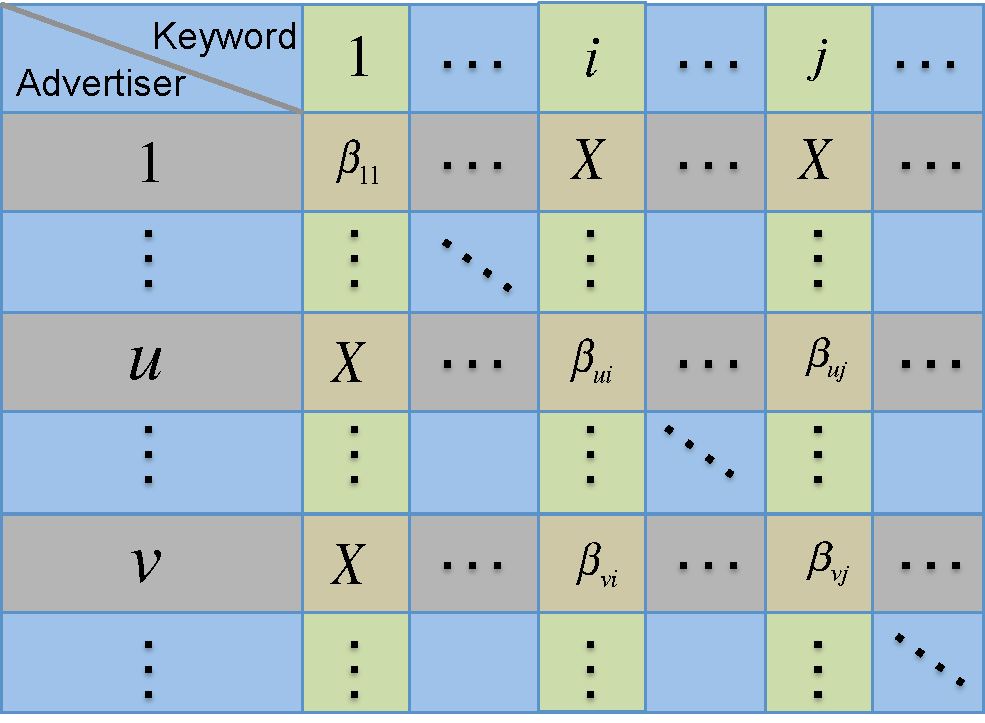
\includegraphics[width=0.35\textwidth]{figures/matrix.pdf}
  \caption{Matrix ??}
  \label{fig:problem-as-matrix}
\end{figure}
We take same settings as other Colleborative Filtering algorithms,
where the input keyword traffic data can be viewed as a matrix, as
shown in Figure~\ref{fig:problem-as-matrix}. Each row represents an
advertisement and each column represents a keyword. If a keyword $i$
is already associated with advertisement $u$, then we have some
observed traffic value $\beta_{ui}$. Otherwise, no value is observed
(noted as $X$). For convenience, we define the notations we will use
through out this paper in Table~\ref{tab:notations}. Specially $u$ and
$v$ will be used for advertisers, while $i$ and $j$ will be used for
keywords.

\begin{table}[!ht]
  \centering
  \begin{tabular}{|l|l|}
    \hline
    Notation & Description \\ \hline
    $N_a$ & total number of advertisements \\ \hline
    $N_k$ & total number of keywords \\ \hline
    $u$ & the $u$th advertisement, $u\in [1,N_a]$\\ \hline
    $i$ & the $i$th keywords, $i\in [1,N_k]$\\ \hline
    $\Lambda$ & missing values in data matrix $M$\\ \hline
    $\Lambda_{(*,i)}$  & missing values in the $i$th column of matrix $M$\\ \hline
    $\Lambda_{(u,*)}$ & missing values in the $u$th row of matrix $M$\\ \hline
    $\Gamma$ & observed (known) values in the matrix $M$\\ \hline
    $\Gamma_{(*,i)}$ & observed values in the $i$th column of matrix $M$\\ \hline
    $\Gamma_{(u,*)}$& observed values in the $u$th row of matrix $M$\\     \hline
    $\beta_{ui}$& observed value for cell ($u$,$i$) of matrix $M$\\ \hline
    $\hat{\beta}_{ui}$& model estimated value for cell ($u$,$i$) of matrix $M$\\ \hline
  \end{tabular}
  \caption{Notations for {\sppan} Model}
\label{tab:notations}
\end{table}

The quality of the model is evaluated by the standard root mean square
error (RMSE), which is
\[
\sqrt{\frac{1}{N_a \times N_k}\sum_u \sum_i \left(\beta_{ui}-\hat{\beta}_{ui}\right)^2}
\]

\section{Similarity Amplifier Network }
\label{sec:model}

We first give an overview of our solution, and then describe its
deployment in production.

\subsection{Model Intuition} 
\label{sec:model_intuition}

Our model is inspired by the similar idea of collaborative filtering
that the preference of a user on an item is predicted based on the
preferences of other users with similar interests.  There are mainly
two categories of collaborative filtering, either in user-centric or
item-centric manner:
\begin{itemize}
\item item-based collaborative filtering: build an item-item matrix
  determining relationships between pairs of items, then infer the
  tastes of the current user by examining the matrix and matching that
  user's data, e.g. users who bought x also bought y
\item user-based collaborative filtering: look for users who share the
  same rating patterns with the active user (the user whom the
  prediction is for). Then use the ratings from those like-minded
  users found in step 1 to calculate a prediction for the active user,
  e.g. people also looks at the following items
\end{itemize}
Both item-based and user-based models are trying to emphasize only one
perspective of the problem, but did not consider the correlation cross
them.

\textit{ Is it possible to use the information from both dimensions to
  further improve the model's prediction performance? }

The answer is positive. Why?  because the two dimention model further
amplify the effect of homogeneous cross both item and users, which we
named as {\it Homogeneous Amplifying Effect} in this
paper. \textcolor{red}{NEED MORE EXPLAINATION IN HUMAN LANGUAGE}

The main idea of our model is illustrated by
Figure~\ref{fig:sppan-idea}, where $u,v,w$ are advertisements, and
$i,j,k$ are keywords, and the value in each cell is the average daily
clicks for the corresponding advertisement from the keyword query.
Let's say we want to predict the average daily click value if we want
to add keyword $k$ to advertisement $v$. For keyword pair $k$ and $j$,
we observed ratio $20/12$ in advertisement $u$ and $5/18$ in
advertisement $w$. If we can derive the performance ratio between $k$
and $j$ in advertisement $v$, then we can make use of $j$'s observed
daily average clicks in $v$ to give one estimate of $k$'s daily
average clicks in $v$. To do so, we introduce a set of parameters
called {\em similarity}, one for each pair of advertisements, to
capture how similar the performance ratios will be between
advertisements. Let $\similarity{u}{v},\similarity{v}{w}$ be the
similarity between $u,v$ and $v,w$ respectively. The estimate given by
keyword pair $k,j$ can be expressed as
\[ 6\times \left(\frac{20}{12}\times\similarity{u}{v} + \frac{5}{18}\times\similarity{v}{w} \right)\div \left(\similarity{u}{v} + \similarity{v}{w} \right) \]
Similarly, we can have another estimate by keyword pair $k,i$, which is
\[ 9\times \left(\frac{20}{5}\times\similarity{u}{v} + \frac{5}{22}\times\similarity{v}{w} \right)\div \left(\similarity{u}{v} + \similarity{v}{w} \right) \]

\begin{figure}[!ht]
  \centering
  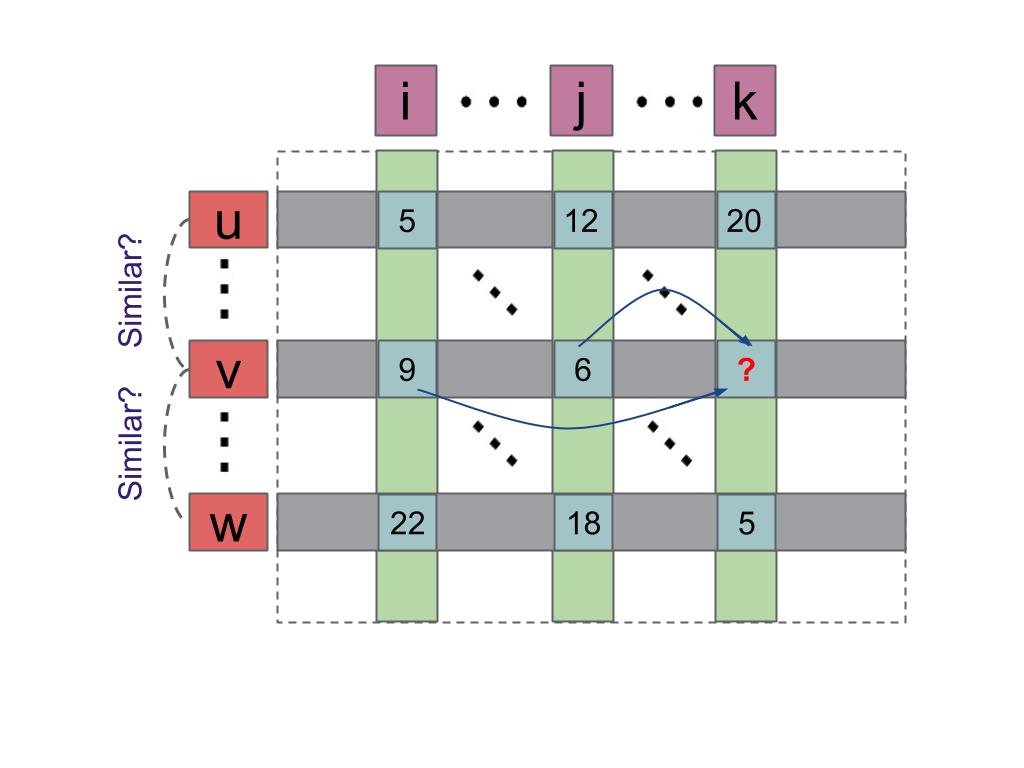
\includegraphics[width=0.5\textwidth]{figures/example.jpg}
  \caption{High level idea of SPPAN model.}
  \label{fig:sppan-idea}
\end{figure}

Now how do we combine these estimates? We introduce another set of
parameters called {\em confidence}, one for each pair of
keywords. Therefore, the final estimate can be represented as the
linear combination of the above two estimates, weighted by the
confidences of keyword pairs $k,j$ and $k,i$. All the parameters are
learned from SPPAN trainer by gradient descent algorithm. They will be
introduced later in Section \ref{sec:simi_graph} and \ref{sec:pag}.

\subsection{Modeling Similarity Amplifier Network} 
\label{sec:model_san}

Under the context of advertisement traffic estimation, it can be interpreted as:
\begin{itemize}
\item Similar advertisers are likely to have similar traffic ratios
  between the same pair of keywords, i.e. $\beta_{uj}/\beta_{ui}
  \approx \beta_{vj}/\beta_{vi}$ where $u$ and $v$ are ``similar''
  adgroups.
\item Similar keywords are likely to have similar entry value ratios
  between the same pair of advertisers, i.e. $\beta_{vi}/\beta_{ui}
  \approx \beta_{vj}/\beta_{uj}$ where $i$ and $j$ are ``similar''
  criteria.
\end{itemize}

Table \ref{tab:notations} shows the notations in this paper, specially
$u$ and $v$ will be used for advertisers, while $i$ and $j$ will be
used for keywords.

\begin{table}[!ht]
\centering
	\begin{tabular}{|l|l|}
	\hline
    Notation & Description \\ \hline
	$N_a$ & total number of advertisements \\ \hline
	$N_k$ & total number of keywords \\ \hline
	$a_u$ & the $u$th advertisement, $u\in [1,N_a]$\\ \hline
    $k_i$ & the $i$th keywords, $i\in [1,N_k]$\\ \hline
    $\Lambda$ & missing values in data matrix $M$\\ \hline
    $\Lambda_{(*,i)}$  & missing values in the $i$th column of matrix $M$\\ \hline
    $\Lambda_{(u,*)}$ & missing values in the $u$th row of matrix $M$\\ \hline
    $\Gamma$ & observed (known) values in the matrix $M$\\ \hline
    $\Gamma_{(*,i)}$ & observed values in the $i$th column of matrix $M$\\ \hline
    $\Gamma_{(u,*)}$& observed values in the $u$th row of matrix $M$\\     \hline
	\end{tabular}
	\caption{Notations for SPAN Model}
\label{tab:notations}
\end{table}

\subsubsection{Similarity Graph}
\label{sec:simi_graph}
Similarity Graph is the graph which describes the similarity between
different advertisers. To be more specific, it is a complete
undirected graph $G_{\mbox{sim}}$ $=<V,E>$, where $V$ is the set of
all the advertisers $V=\{a_1,a_2,...,a_{N_a}\}$. For each edge in $R$,
there is a value which represents how similar the corresponding two
advertisers are with each other. Let $\theta_{uv}$ denote the
similarity between advertiser $a_u$ and $a_v$.

\begin{comment}
% this graph does not provide much useful information, but a normal graph structure
 Figure~\ref{fig:sim-graph} shows an example fragment of the Similarity Graph.
\begin{figure}[!ht]
  \centering
  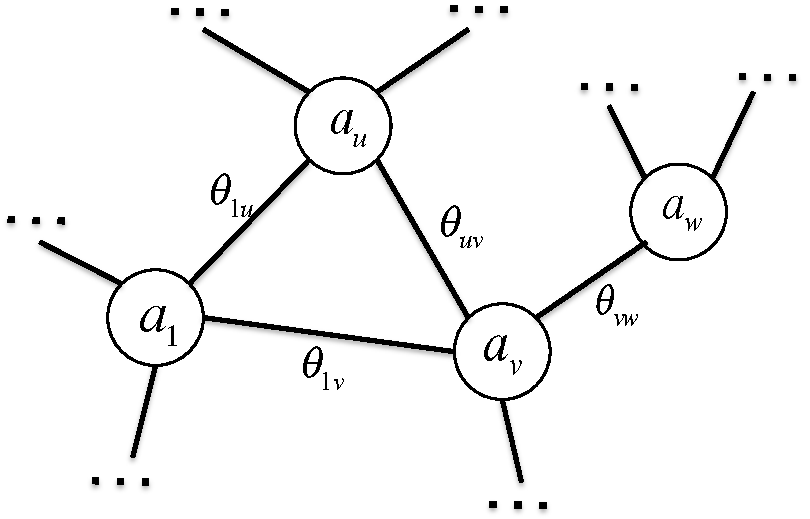
\includegraphics[width=0.35\textwidth]{figures/sim_graph.pdf}
  \caption{Similarity Graph}
  \label{fig:sim-graph}
\end{figure}
\end{comment}

\subsubsection{Pairwise Amplifier Graph}
\label{sec:pag}
Pairwise Amplifier Graph contains all the ratio information between
different pairs of keywords. It is defined as a directed graph
$G_{\mbox{amp}}=<V,E>$, where $V$ contains all the keywords
$V=\{k_1,k_2,...,k_{N_k}\}$, and $E$ contains all pairs of keywords
that have been targeted concurrently in at least one advertiser,
$E=\{(k_i,k_j)~|~i\in [1,N_k],j$ $\in [1,N_k],\exists u\in $ $
[1,N_a]\mbox{ s.t. }\beta_{ui},$ $\beta_{uj}\in \Gamma\}$. For each
edge $(k_i,k_j)\in E$, there are a corresponding confidence value
$conf_{ij}$ and an amplifier set $amp_{ij}=\{(a_u,\gain{u}{ij})~|~u\in
[1,N_a],\beta_{ui},\beta_{uj}\in \Gamma\} \cup \{(a_0,c_{ij})\}$,
where $\gain{u}{ij}=\beta_{uj}/\beta_{ui}$, and $(a_0,c_{ij})$ are
just the bias terms which we will use later in the model.

\begin{comment}
 Figure~\ref{fig:amp-graph} shows an example fragment of the Pairwise
 Amplifier Graph.

\begin{figure}[!ht]
  \centering
  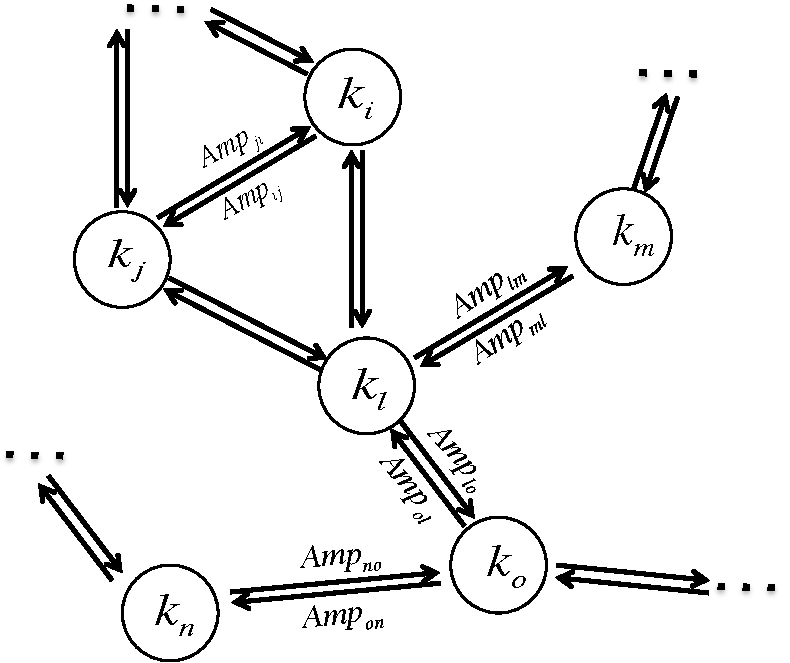
\includegraphics[width=0.35\textwidth]{figures/amp_graph.pdf}
  \caption{Pairwise Amplifier Graph}
  \label{fig:amp-graph}
\end{figure}
\end{comment}

%%%%%%%%%%%%%%%%%%%%%%%%%%%%%%%%%%%%%%%%%%%%%%%%%%%%%%%%%%
\section{Training a Simplify Amplify Network}
\label{sec:trainer}

\begin{figure}[!ht]
  \centering  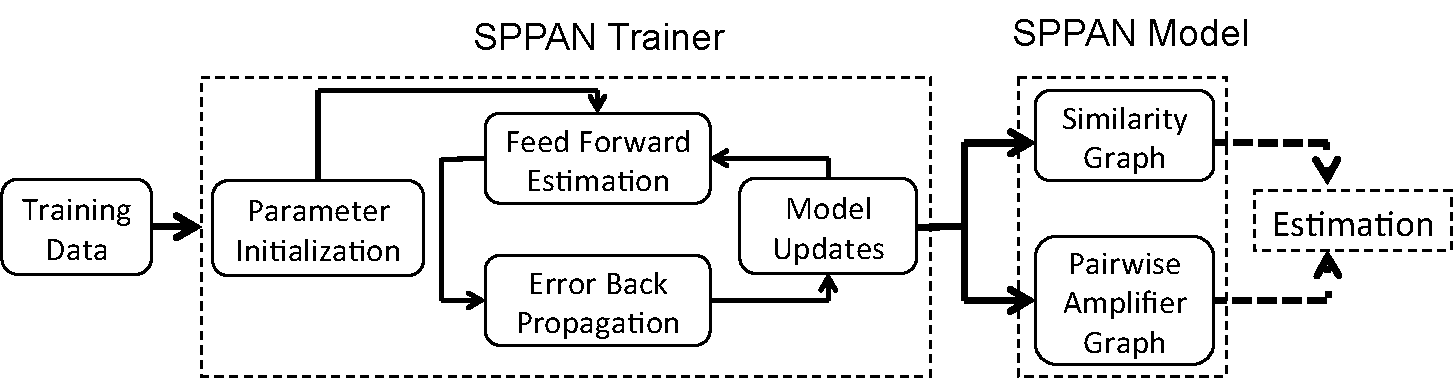
\includegraphics[width=0.5\textwidth]{figures/model.pdf}
  \caption{SPAN system overview.}
  \label{fig:model}
\end{figure}

The mainl workflow of SPAN model is summarized in
Figure~\ref{fig:model}.  The training dataset can be regarded as a
sparse 2D matrix with known entries shown in Figure
\ref{fig:problem-as-matrix}.  Given the training dataset, the training
process starts with a set of initial parameters, then there is an
update loop between feeding forward estimation and backword
propogation, in which {\it Feed Forward Estimation} uses the given
data points to estimate the value of a target entry.  {\it Error Back
  Propagation} updates current model parameters.  The training process
is in an incrementally update way, and generate the final model which
is composed of similarity graph and pairwise amplifier graph. The
learned SPAN model will be directly used to estimate missing values.
In the following sections, we will discuss each component in details.

%The "SPPAN Trainer" is the training module of our proposed SPPAN
%model, which will be further discussed in
%Section~\ref{sec:trainer}. % The output of "SPPAN Trainer" is the
%trained SPPAN model which consists of two major components in SPPAN
%model:(1) Similarity Graph, and (2) Pairwise Amplifier Graph. We will
%cover both components in Section \ref{sec:simi_graph} and
%\ref{sec:pag}.  Consider the advertisement traffic estimation problem
%described in Section~\ref{sec:intro}, The trained SPPAN model will be
%used to estimate the values of interested missing entries in that
%matrix.

\subsection{Feed Forward Estimation}
\label{sec:ffe}

\begin{figure}[!ht]
  \centering
  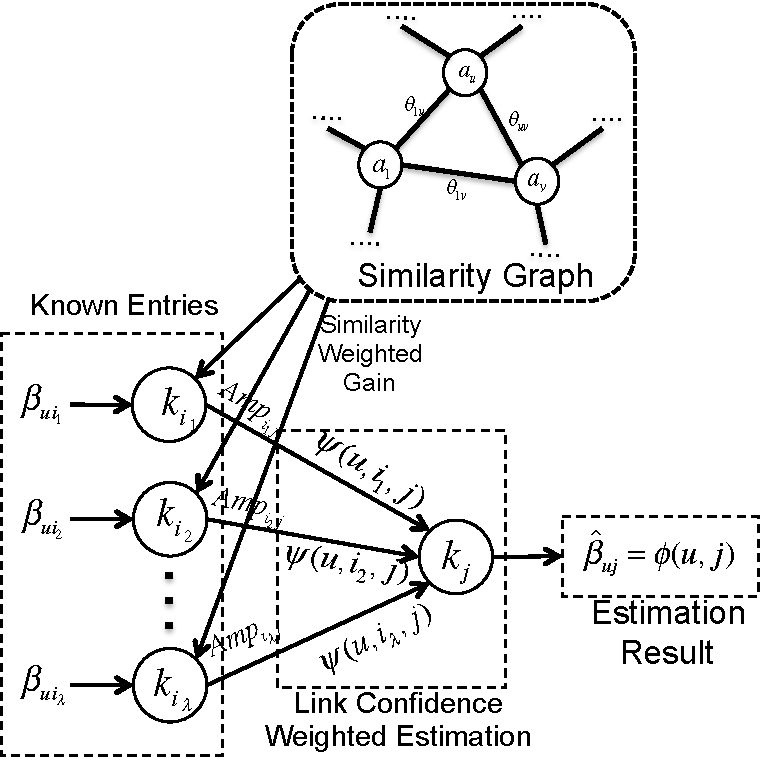
\includegraphics[width=0.43\textwidth]{figures/trainer_feedforward.pdf}
  \caption{Feed Forward Estimation}
  \label{fig:trainer-feedforward}
\end{figure}

\textcolor{red}{ADD MORE DESCRIPTION HERE, need to understand what is
  two layers calculation units? ...}

Given particular values for initial parameters and the inputs data, to
predict parameter settings that minimize the error, our model uses
feed-forward network: the inputs feed into a layer of hidden units,
which can feed into layers of more hidden units, which eventually feed
into the output layer. Each of the hidden units is a squashed linear
function of its inputs.

Our SPAN model uses known entry values $\{\beta_{ui_1}, \beta_{ui_2},
\cdots, \beta_{ui_\lambda}\}$ (where $\lambda$ is the number of known
entry values of advertiser $u$) to estimate the value of target entry
$\beta_{uj}$.  It uses feed forward network to estimate the parameters
in a layer-by-layer way: takes known entry values as inputs, it goes
through a two layers of calculation units to get the final estimated
result.  Similarity weighted sum of entry estimation (in Equation
\ref{eq:feedforward_1}.) and a link confidence weighted sum of entry
estimation (in Equation \ref{eq:feedforward_2} ) are used to estimate
the value of an unknown entry $\beta_{uj} \in \Lambda$ .

As shown in Figure \ref{fig:trainer-feedforward}, the first layer make
estimation of target $\beta_{uj}$ using $\{\beta_{ui_1}, \beta_{ui_2},
\cdots, \beta_{ui_\lambda}\}$ separately with equation
\ref{eq:feedforward_2}, which generates $\lambda$ output estimated
values. The second layer takes all the output estimations from the
first layer $\{\psi(u,i_1,j),\psi(u,i_2,j),\cdots
\psi(u,i_\lambda,j)\}$ as inputs to calculate the final prediction
using equation \ref{eq:feedforward_1}.

\newcommand{\wconf}[3]{\sum\limits_{{#2}:\beta_{{#1}{#2}}\in\Gamma_{({#1},*)}} \confi{{#2}{#3}}\cdot \psi({#1},{#2},{#3})}
\newcommand{\sconf}[3]{\sum\limits_{{#2}:\beta_{{#1}{#2}}\in\Gamma_{({#1},*)}} \confi{{#2}{#3}}}

\newcommand{\wtheta}[2]{\sum \limits_{{#2}:(a_{#2},\gain{{#2}}{ij})\in\amp{ij}} \theta_{{#1}{#2}} \cdot \gain{{#2}}{ij}}
\newcommand{\stheta}[2]{\sum \limits_{{#2}:(a_{#2},\gain{{#2}}{ij})\in\amp{ij}} \theta_{{#1}{#2}}}

\begin{equation}
  \label{eq:feedforward_2}
  \begin{cases}   
    \psi (u,i,j) = \frac{\sum \limits_{v\in V} \theta_{uv} \cdot \gain{{v}}{ij}}{\sum \limits_{v\in V} \theta_{uv}} \cdot \beta_{ui} \\
    V=\{v|(a_{v},\gain{{v}}{ij})\in\amp{ij}\}
   \end{cases}
\end{equation}

\begin{equation}
  \label{eq:feedforward_1}
  \begin{cases}    \hat{\beta}_{uj}=\phi(u,j)=\frac{\sum\limits_{i\in I} \confi{ij}\cdot \psi(u,i,j)}{\sum\limits_{i\in I} \confi{ij}} \\
  	    I=\{i|\beta_{ui}\in\Gamma_{(u,*)}\}
  \end{cases}
\end{equation}

\subsection{Error Back Propagation}
\label{sec:bp}

In Feed Forward Estimation process , we assume the similarity
parameters of advertiser pairs ( in Similarity Graph) and the link
confidence parameters in the Pairwise Amplifier Graph are
given. Indeed the model needs to learn these parameters from the
training dataset using error back proprgation.  The idea of error back
propagation is very similar to artificial neural networks: for an
entry in the training dataset, we hide this entry from the rest of the
training dataset and use the feed forward estimation algorithm in
Section~\ref{sec:ffe} to estimate its value with the rest of the
training dataset. Then we compare the true value of that entry with
current estimation, and back propagate the estimation error (the
deviation from estimated value to the true value) to update the
parameters.  The idea is shown in
Figure~\ref{fig:trainer-train-entry}.  Gradient descent method
\cite{?} is used to optimize the model parameters, which calculates
the gradient of a loss function with respects to all the weights in
the network. The gradient is fed to the optimization method which in
turn uses it to update the weights, in an attempt to minimize the loss
function.

Before developing the parameter update function, we need to calculate
the derivative of the squared error function with respect to all the
parameters in SPAN model, including both
$\{\theta_{uv}\}_{u,v\in[1,N_a]}$ and
$\{\confi{ij}\}_{(i,j):(k_i,k_j)\in E(G_{amp})}$.

The objective function of the parameter optimization problem is shown
in Equation \ref{eq:sum-square-err}, which is the sum of squared
estimation error for all the entries in the training dataset.

\begin{figure}[!ht]
  \centering
  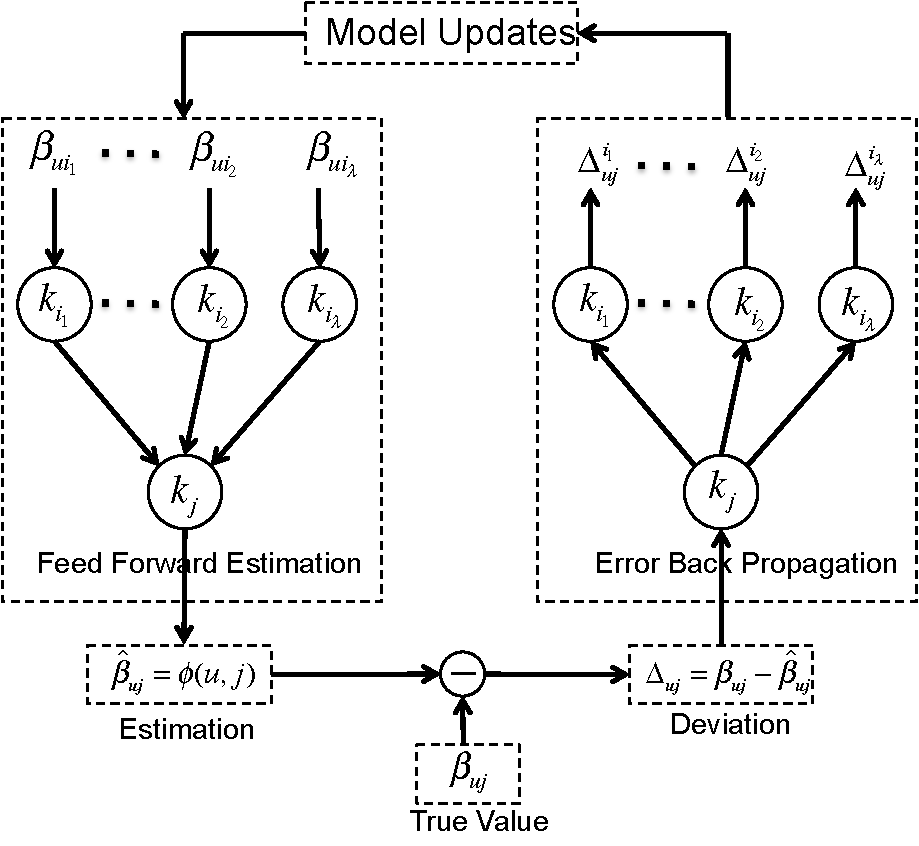
\includegraphics[width=0.49\textwidth]{figures/trainer_train_entry.pdf}
  \caption{The Loop of the Parameter Update}
  \label{fig:trainer-train-entry}
\end{figure}

\begin{equation}
  \label{eq:sum-square-err}
  \begin{aligned}
    J &= \frac{1}{2} \sum_{u,i:\beta_{ui}\in\Gamma} \left(\beta_{ui}-\hat{\beta}_{ui}\right)^2 \\
    &= \frac{1}{2} \sum_{u,i:\beta_{ui}\in\Gamma} \left(\beta_{ui}-\phi(u,i)\right)^2 \\
    &= \frac{1}{2} \sum_{u,i:\beta_{ui}\in\Gamma} \Delta^2_{ui}
  \end{aligned}
\end{equation}

Where $\beta_{ui}$ is the true value, and $\hat{\beta}_{ui}=\phi(u,i)$
is the estimated value given by Feed Forward Estimation algorithm we
described in Section~\ref{sec:ffe}. The factor of $\frac{1}{2}$ at the
beginning of the objective function is a constant factor which would
simplify the expression after the differentiation operation. Noted
that an arbitrary learning rate factor will be multiplied with this
expression in our later learning process, so that it doesn't make any
differences if a constant coefficient is introduced here.

With Equation \ref{eq:feedforward_2}, \ref{eq:feedforward_1} and
\ref{eq:sum-square-err}, the derivatives of our objective function
with respect to parameters $\{\theta_{uv}\}_{u,v\in[1,N_a]}$ and
$\{\confi{ij}\}_{i,j\in[1,N_k]}$ are
\[
\pa{J}{\theta_{uv}} = \sum_{j:\beta_{uj},\beta_{vj}\in\Gamma} \pa{\left[\frac{1}{2}\left(\beta_{uj}-\hat{\beta}_{uj}\right)^2\right]}{\theta_{uv}}
\]
and
\[
\pa{J}{\confi{ij}} = \sum_{u:(a_u,\gain{u}{ij})\in\amp{ij}} \pa{\left[\frac{1}{2}\left(\beta_{uj}-\hat{\beta}_{uj}\right)^2\right]} {\confi{ij}}
\]

With further formula deductions, we can have Equation
\ref{eq:simi_dev} as the derivative result of the objective function
with respect to $\{\theta_{uv}\}_{u,v\in[1,N_a]}$, and Equation
\ref{eq:conf_dev} as the derivative result of the objective function
with respect to $\{\confi{ij}\}_{i,j\in[1,N_k]}$.

\begin{equation}
  \label{eq:simi_dev}
  \begin{cases}
    \pa{J}{\theta_{uv}}=\sum\limits_{j\in J} \sum\limits_{i\in I} \frac{-\Delta_{uj}^{i}}{\sum \limits_{v'\in V} \theta_{{u}{v'}}}  \left(\gain{v}{ij}\cdot\beta_{ui}- \psi(u,i,j)\right) \\
    J=\{j|\beta_{uj},\beta_{vj}\in\Gamma\} \\
    I=\{i|\beta_{ui}\in\Gamma_{(u,*)}\} \\
    V=\{v|(a_{v},\gain{{v}}{ij})\in \amp{ij}\}
  \end{cases}
\end{equation}

\begin{equation}
  \label{eq:conf_dev}
  \begin{cases}
    \pa{J}{\confi{ij}}=\sum\limits_{u\in U} \left[ -\frac{\Delta_{uj}}{\sum\limits_{i'\in I} \confi{{i'}{j}}} \left(\psi(u,i,j) - \phi(u,j)\right) \right] \\
    U=\{u|(a_u,\gain{u}{ij})\in\amp{ij}\} \\
    I=\{i:\beta_{{u}{i}}\in\Gamma_{({u},*)}\}
  \end{cases}
\end{equation}

where $\Delta_{uj}$ is the estimation error and $\Delta_{uj}^{i}$ is
back propagated error, their expressions are given by
Equation~\ref{eq:derivative_condition}.

\begin{equation}
  \label{eq:derivative_condition}
  \begin{cases}
    \Delta_{uj}=\beta_{uj}-\hat{\beta}_{uj}\\
    \Delta_{uj}^{i}=\frac{\confi{ij}}{\sconf{u}{i'}{j}}\cdot \Delta_{uj}
  \end{cases}
\end{equation}

With the derivatives and back propagated errors given by Equation
\ref{eq:simi_dev}, \ref{eq:conf_dev} and
\ref{eq:derivative_condition}, we can update the parameter of SPPAN
model in the Similarity Graph and the Pairwise Amplifier Graph using
the gradient descent approach. Given a specific learning rate $\eta$,
the changes of model parameters are equal to the product of the
learning rate and the corresponding gradient value, multiplied by
-1. Therefore, the parameter update function for training target
$\beta_{uj}$ can be expressed in Equation \ref{eq:gradient descent}.

\begin{equation}
  \label{eq:gradient descent}
  \begin{cases}
    \confi{ij} := \confi{ij}-\eta \cdot \pa{J}{\confi{ij}}\\
    \theta_{uv} := \theta_{uv} -\eta \cdot \pa{J}{\theta_{uv}}
  \end{cases}
\end{equation}

\noindent where $\pa{J}{\confi{ij}}$ and $\pa{J}{\theta_{uv}}$ are
given by Equation \ref{eq:simi_dev}, \ref{eq:conf_dev} and
\ref{eq:derivative_condition}. Figure \ref{fig:trainer-train-entry}
shows the parameter update loop of the Feed Forward Estimation and the
Error Back Propagation for a training target entry $\beta_{uj}$.

\subsection{Training Algorithm for SPAN model}
Combining the Feed Forward Estimation and Error Back Propagation, The
training algorithm for SPPAN model can be summarized in Algorithm
\ref{alg:training}.

The stop criterion for the training algorithm is a training error
threshold: the training will stop if the training error drops to a
specific value. Other criterion may also be used, such as maximum
iteration number\cite{?}, error reduction rate threshold\cite{?}, the
convergence of the parameters\cite{?} and so on.

The training algorithm generates final SPAN model, which includes the
Similarity Graph and Pairwise Amplifier Graph. To estimate unknown
entries, we can just follow the Feed Forward Estimation described in
Section \ref{sec:ffe}, using the well-trained Similarity Graph and
Pairwise Amplifier Graph.


\begin{algorithm}
  \KwData{The set of given/known entries $\Gamma$ in matrix $M$\\
    ~~~~~~~~~Learning rate $\eta$\\
  }
  \KwResult{$\{\theta_{uv}\}_{u,v\in[1,N_a]}$ in adgroups similarity graph \\
    ~~~~~~~~~~~~$\{\confi{ij}\}_{(i,j):(k_i,k_j)\in E(G_{amp})}$ in criteria pairwise amplifier graph
  }
  \textbf{Initialization:}\\
  \begin{itemize}
  \item initialize the pairwise amplifier set
    $Amp_{ij}=\{(a_u,\gain{u}{ij})~|~u\in
    [1,N_a],\beta_{ui},\beta_{uj}\in \Gamma\} \cup \{(a_0,c_{ij})\}$
    using $\gain{u}{ij}=\beta_{uj}/\beta_{ui}$
  \item initialize parameters $\{\theta_{uv}\}$ in adgroup similarity
    graph using small random numbers when encountered.
  \item initialize parameters $\{\confi{ij}\}$ in criteria pairwise
    amplifier graph using small random numbers when encountered.
  \end{itemize}
  \Begin{
    \While{stop criterion not meet}{
      \For{each $\beta_{uj}$ in $\Gamma$}{
  \tcc{ SPPAN Model feed forward estimation of training example $\beta_{uj}$} 
  \tcc{with Equation~\ref{eq:feedforward_2} and \ref{eq:feedforward_1}}
  $\hat{\beta}_{uj}=FeedForwardEstimation(\mbox{SPPAN Model},u,j)$  \\
  \tcc{error back propagation using Equation~\ref{eq:derivative_condition}}
  $(\Delta_{uj},\{\Delta_{uj}^{i}\})=ErrorBackPropagation(\mbox{SPPAN Model},u,j,\hat{\beta}_{uj})$ \\
  \tcc{update SPPAN model using gradient descent Equation \ref{eq:simi_dev}, \ref{eq:conf_dev} and \ref{eq:derivative_condition}}
  $update(\mbox{SPPAN Model},\Delta_{uj},\{\Delta_{uj}^{i}\})$
      }
    }
    return (\mbox{SPPAN Model})
  }
  \caption{Training Algorithm for SPPAN Model}
  \label{alg:training}
\end{algorithm}

\subsection{Handling Large Scale  Data}
Algorithm \ref{alg:training} works well in most cases. However, as the
data set become much bigger and less sparse, the iterative process of
error back propagation based parameter update for SPPAN model often
take a great deal of time to completely go through the whole training
set.  Another advantage of our model is that it can handle large scale
sparse data in an effective way. As we can see from Algorithm
\ref{alg:training}, the SPPAN model updates can use different
independent training samplesr. Thus, map-reduce techniques can be used
to greatly decrease the amount of time that the training algorithm
takes to converge.

For each training iteration, the mapping part can takes each training
example separately and executes the feed forward and error backward
propagation in parallel to generate model updates. Then, the updates
for all the parameters of SPPAN model are summed up in the reducing
units. At the end of each iteration, the SPPAN model can be updated
using the outputs from the reducing unites. This process continues
until the stop criterion is met.


\subsection{Handling Extreme Sparse Data}

\textcolor{red}{add a section about how to handle extreme sparse data,
  explain why your model can handle extrem sparse data}


\section{System Architecture}
\label{sec:archi}
This section explains how we implement our SPAN model and deploy into Google's Adsense system.
\textcolor{red} {add one architecture photo,  add some description about how does the systme work}


\section{Experiments}
\label{sec:exp}

\textcolor{red}{ please add/revise necessary part}

In this section, we report our experiments on evaluating the
effectiveness and robustness of the proposed framework.  The
evaluation is based on adsense data collected from Google's adsense
system over a 1-year period from ....

In our study, we partition the dataset into training and testing
sets. Using the training set, we first build the SPAN models presented
in Section \cite{model}.  Then for each advertisement in the testing
set, we apply the algorithms introduced in Section ?? to predict the
recommendation result for..

We implement the proposed {\sppan} model in both Python and C++ that
can run on a single machine, also a parallel C++ version based on
Map-reduce.  To evaluate the effectiveness of our system, we use the
Python version to compare its performance with a baseline method and
two Nonnegative Matrix Factorization based methods provided by nimfa
Python library \cite{ZitnikZ12}.

\begin{itemize} \itemsep -2pt
\item {\em Baseline}: The baseline method is giving prediction simply
  based on the average value in the training set.
\item {\em LSNMF(??? stands for?)}: based on alternating nonnegative least
  squares matrix factorization using projected gradient method for
  subproblems\cite{lin2007projected}.
\item {\em NMF(???stands for????)}: based on Standard nonnegative matrix
  factorization with Euclidean / Kullback-Leibler update equations and
  Frobenius / divergence / connectivity cost
  functions\cite{lee2001algorithms, brunet2004metagenes}.
\end{itemize}

%To provide more interpretable experiment results and for data privacy
%considerations, we show the performance result of NMF, LSNMF and
%{\sppan} as their relative performance to the baseline method in all
%the following subsections. The results of the evaluation experiments
%show salient advantages of {\sppan} model compare to those two NMF
%based methods:

Our experiments will demonstrate:
\begin{itemize} \itemsep -2pt
\item {Better Prediction Accuracy} The matrix factorization based
  methods LSNMF and NMF are not handling the present extreme sparse
  click-through rate (CTR) data set very well. Their prediction
  accuracy is even worse than the baseline method.
\item {Lower Error Rate} In terms of the training and testing error
  (Root-mean-square deviation), {\sppan} model performs more than
  $65\%$ and $40\%$ better than the matrix factorization based
  methods, and around $60\%$ and $30\%$ better than the baseline
  method.
\item {Balanced Error Distribution} {\sppan} model has a normal error
  distribution centered at 0, which means a balanced estimation; while
  LSNMF and NMF have biased error distributions that are constantly
  under estimating.
\end{itemize}

\subsection{Data Description}
\label{sec:data_desc}
Our evaluation experiments are performed on a click-through rate (CTR)
dataset generated from Google Adsense, which was collected with
appropriate end-user license agreement and was fully anonymized
without any retrievable personally identifiable information.

The CTR data set can be considered as a 2D matrix shown in Figure
\ref{fig:problem-as-matrix}, where each row represents an advertiser
and each column represent a target keyword. The value of each matrix
entry in Figure \ref{fig:problem-as-matrix} is the weekly average CTR
that we observed for the corresponding advertiser on that specific
keyword.

The whole dataset is extremely sparse because there are hundreds of
thousands of different keywords but advertisers usually only target a
very few of them. To be more specific, the dataset contains more than
400k different advertisers (number of rows) and 500k keywords (number
of columns), but more than $99.98\%$ entries in the dataset matrix are
missing.

Because the two Nonnegative Matrix Factorization based methods
provided by nimfa cannot handle the entire CTR dataset ($400k \times
500k$ sparse matrix) on a single machine, we random generate a
sub-sampled version of data set in addition to the original one by
going through each entry in the original dataset and only keep that
entry with specified probability. If all the entry for a row
(advertiser) or column (keyword) are dropped, we simply remove that
row (advertiser) or column (keyword) all together. In Table
\ref{tab:data}, we summarized the basic information of both the $10\%$
sub-sampled version and original data set, including the number of
different advertisers, keywords and known CTR entries. It can be seen
that both datasets are extremely sparse with more than $99.98\%$ of
the entries missing.

\begin{table}[!ht]
  \centering
  \begin{tabular}{|c|c|c|}
    \hline	\hline
    Dataset & whole & $10\%$ sub-sampled\\ \hline
    Advertisers & $\sim 400K$ & $\sim 76K$  \\ 
    Keywords & $\sim 511K$ & $\sim 73K$  \\ 
    Known CTR entries &  $\sim 21M$ & $\sim 2M$ \\ \hline
  \end{tabular}`
  \caption{Dataset Description}
  \label{tab:data}
\end{table}

\subsection{Evaluation}
To compare the estimation performance between LSNMF, NMF and {\sppan}
methods, we randomly partition the sub-sampled CTR dataset into a
$95\%$ as training set for model training, and a $5\%$ as testing set
to evaluate the modesl for the entry values.

\subsubsection{Impact of Factorization Matrix Rank Number}
\textcolor{red}{please revise figure 7, make the font larger, both in
  the legend and the y-axis}

\begin{figure}[!ht]
  \centering
  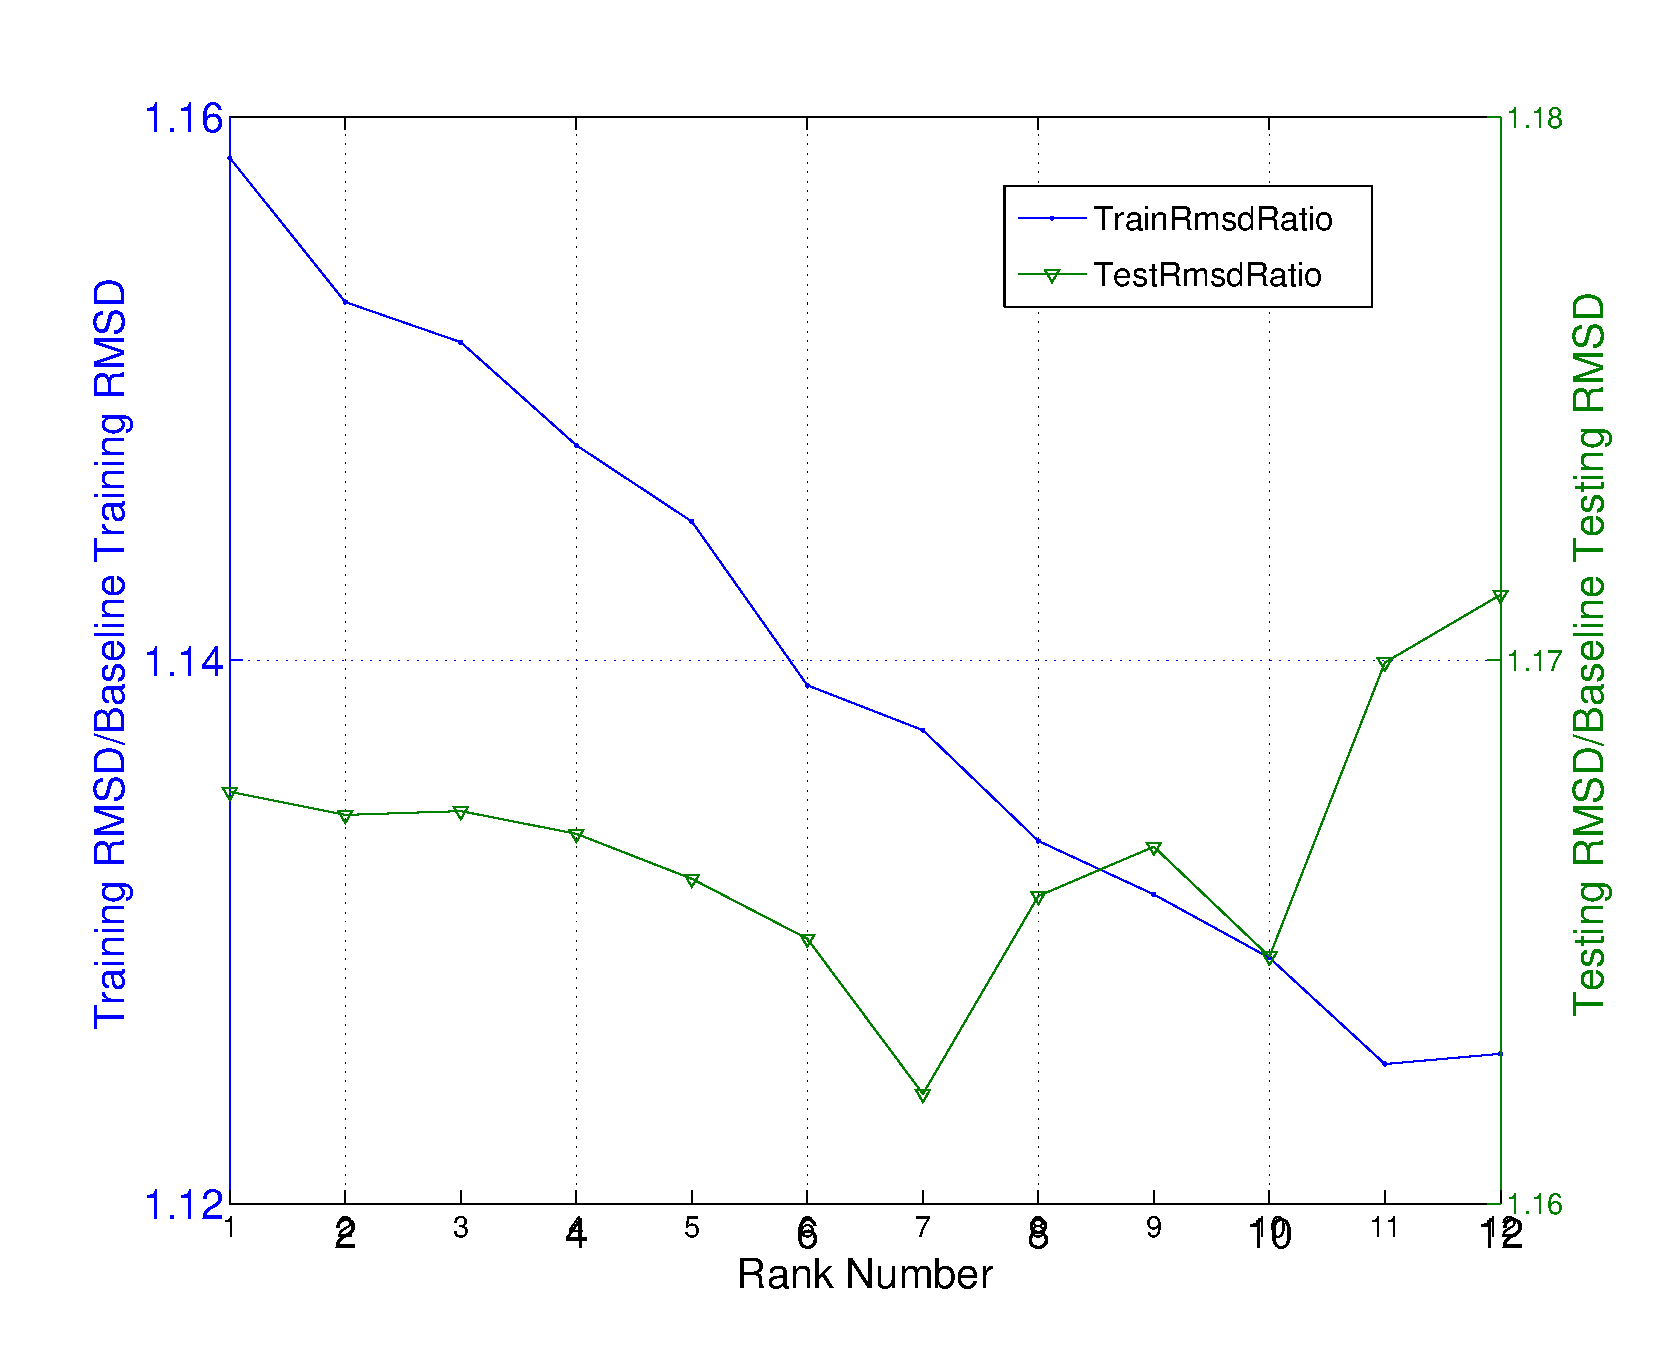
\includegraphics[width=0.4\textwidth]{figures/learning_curve_lsnmf_subsample_relative.eps}
  \caption{LSNMF: Relative Training/Testing Error Versus Rank Number}
  \label{fig:lsnmf_learning}
\end{figure}

For the nonnegative matrix factorization based method LSNMF and NMF,
the ``factorization matrix rank number"\cite{??} need to be specified
before training the model. Using a higher rank number often means a
more complicated matrix model, and more powerful to represent a
dataset, but higher risk of over-fitting. On the other hand, using a
lower rank number means a simpler matrix model, less possible to be
over-fitted but might be too simple to represent the data set.

\textcolor{red}{TODO: change all the names of RMSD to RMSE to be
  consistant with the problem definition} To understand the impact of
rank number in our model, we try to increase the ranking number from 1
to 12 for both LSNMF and NMF methods.  The x-axis is the ranking
number, increasing from 1 to 12, while the y-axis show the ratio of
RMSE value for them with baseline models. Intuitively, the smaller the
RMSE ratio, the better the model is.  As we can see from the results
in Figure \ref{fig:lsnmf_learning}, both of them have a ratio larger
than 1, which means both of them are worse then the baseline model,
indeed they are all overfitting.


\begin{figure}[!ht]
  \centering
  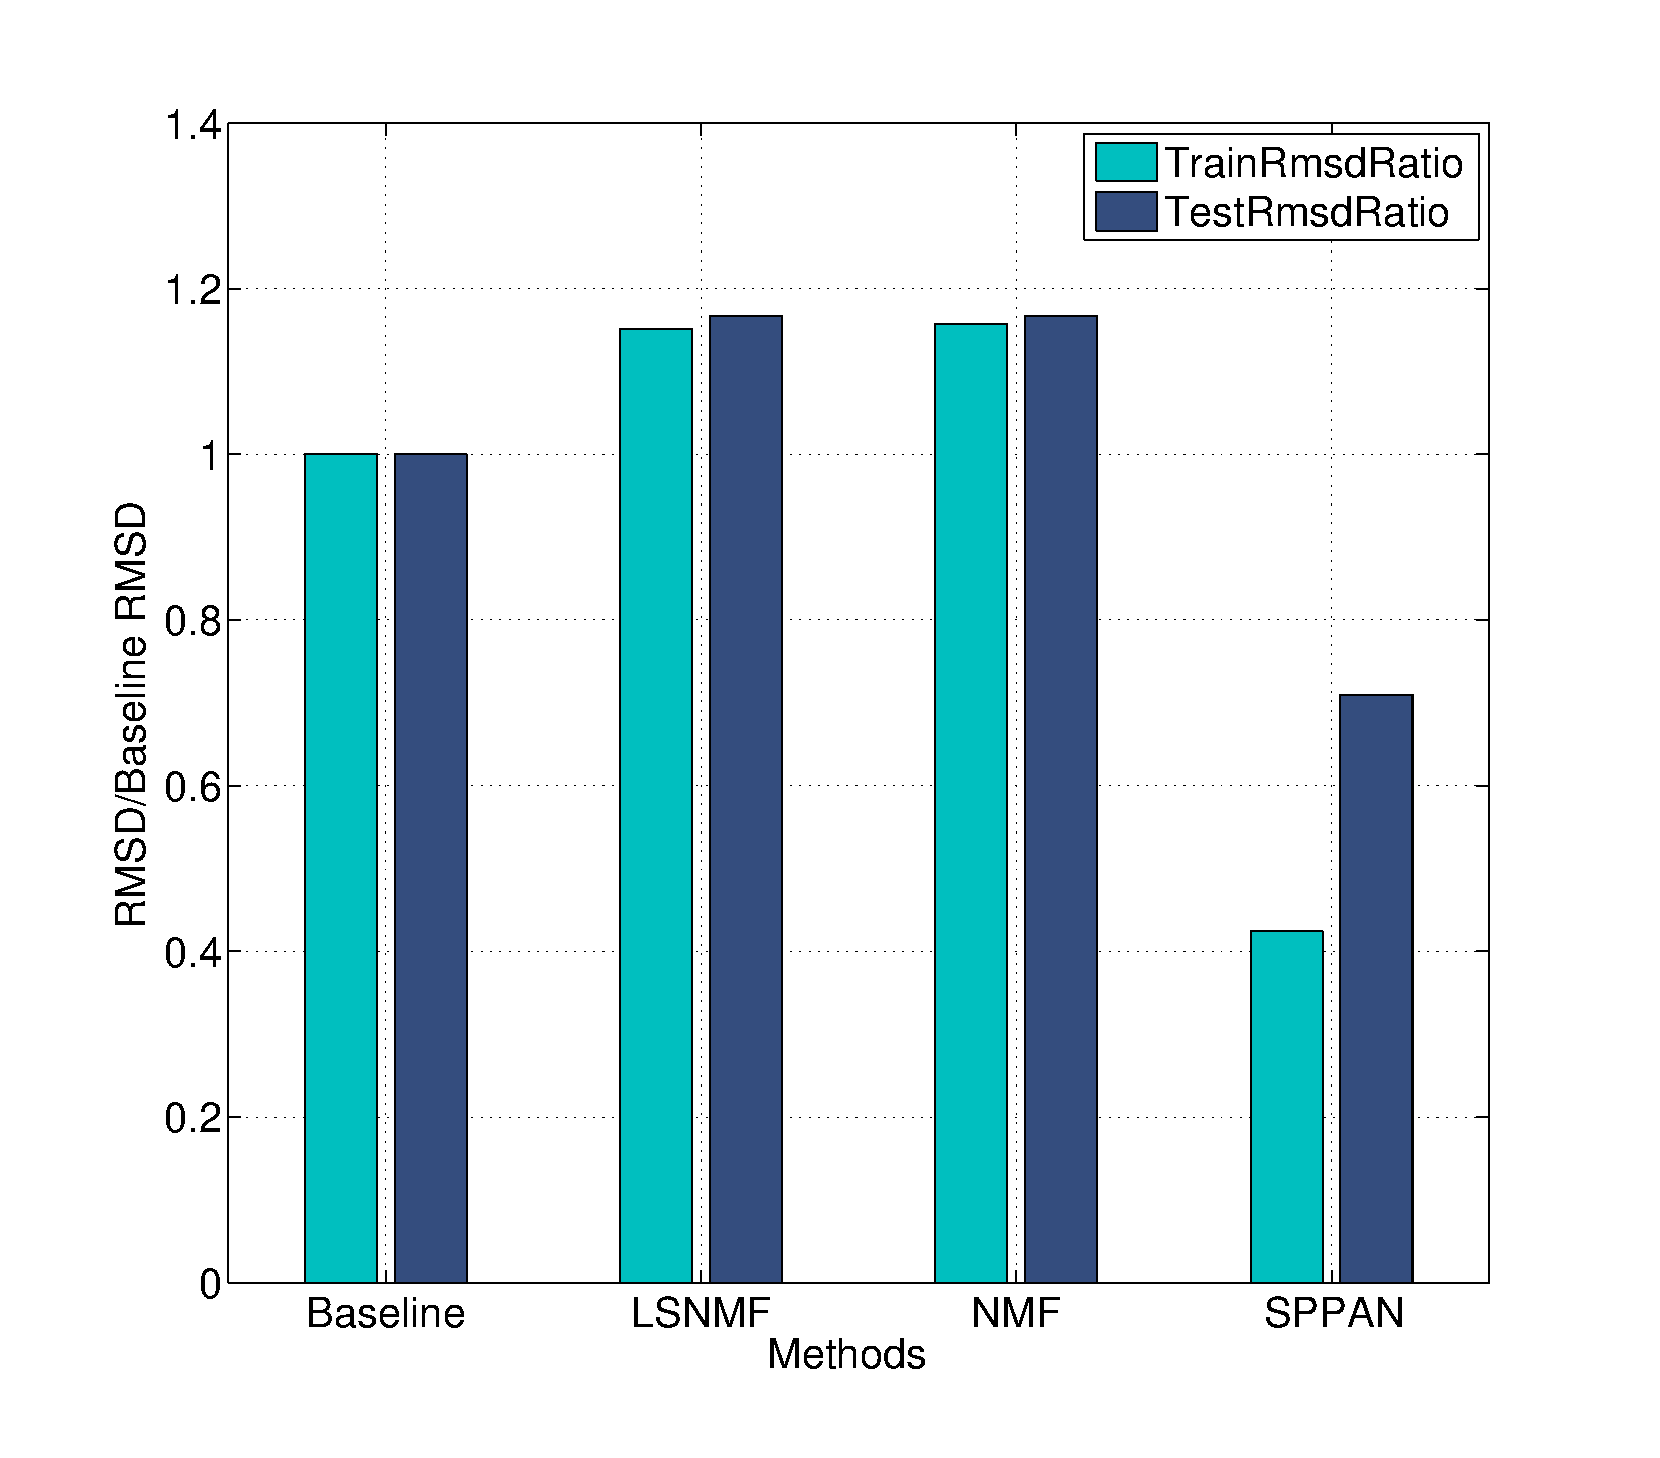
\includegraphics[width=0.45\textwidth]{figures/methos_comparison_all_relative.eps}
  \caption{Compare Relative RMSE Between Different Methods}
  \label{fig:rmsd_compare}
\end{figure}

To compare with our proposed {\sppan} model, we select the best rank
numbers with smallest errors for both LSNMF and NMF, which is 3 and 7
respectively.  \textcolor{red}{In figure 7, it seems that the lowest
  data points are 7, and 10, can u explain?}


\subsubsection{Effectiveness}

As discussed in Section \ref{sec:problem}, RMSE is used to evaluate
the model effectiveness. Furthermore, to have a quatitive comparision
between different modelsl, we use TrainRmsdRatio and TestRmsdRatio to
measure the ratio of training/test RMSD with the baseline
training/testing RMSD, as defined:
\[
TrainRmsdRatio=\frac{\textit{Train RMSD}}{Baseline Train RMSD}
\]
\[
TestRmsdRatio=\frac{\textit{Test RMSD}}{Baseline Test RMSD}
\]

\begin{comment}
The root-mean-square deviation (RMSD) is a measure of the differences
between the estimated value using a model and the true observed
value. It can be expressed using Equation \ref{eq:rmsd_def}, where $n$
is the number of entries that need be to estimated, and
$\hat{\beta_i}$ and $\beta_i$ are the estimated value and observed
value of entry $i$ respectively. The RMSD represents the sample
standard deviation of the differences between estimated values and
observed values \cite{hyndman2006another}.
\begin{equation}
\label{eq:rmsd_def}
RMSD=\sqrt{\frac{\sum\limits_{i=1}^{n}(\hat{\beta_i}-\beta_i)^2}{n}}
\end{equation}

\end{comment}

Figure \ref{fig:rmsd_compare} shows the TrainRmsdRatio and
TestRmsdRatio comparison of baseline, LSNMF, NMF and {\sppan}
model. Even though we chose the best rank numbers for the nonnegative
matrix factorization based methods, they perform even worse than the
baseline method in this extreme sparse case. {\sppan} model, on the
other hand, signigicantly outperforms the Baseline, LSNMF and NMF on
both training and testing RMSD.

\textcolor{red}{TODO: I add a column to the table to indicate the
  improvement \%, please make sure the numbers are correct for the new
  column.  the reason to add that column is as follows: 1) emphasize
  the improvement 2) add valuable informaiton, otherwise table and
  figure are shown the same type of information, without the
  improvement column}

To be more specific, as shown in Table \ref{tab:rmsd_compare} , the
training and testing RMSD of {\sppan} are only around $40\%$ and
$70\%$ of the training and testing RMSD of baseline methods,
respectively. The third and fifth column are the improvement gained by
{\sppan} in training and testing RMSD ratio, they are aroung $35\%$
and $60\%$ improvement of the training and testing RMSD of the matrix
factorization based methods LSNMF and NMF.  It clearly indicates on
average, {\sppan} improves the recommendation efficiency.

\begin{figure}[!ht]
  \centering
  \includegraphics[width=0.42\textwidth]{figures/est_error_hist.eps}
  \caption{Histogram of Estimated Error}
  \label{fig:est_err}
\end{figure}

\begin{table}[!ht]
\centering
\begin{tabular}{|c|c|c|c|c|}
  \hline	\hline
  Method &  TrainRmsdRatio& Improve\%&TestRmsdRatio & Improve\%\\ \hline
  Baseline  & $1$ &$0\%$ & $1$ & $0\%$\\ 
  LSNMF & $1.15$ & $0\%$ & $1.17$ & $-20\%$\\ 
  NMF  & $1.16$   &$0\%$ & $1.17$  & $-30\%$\\ 
  {\sppan}  & $0.42$  &$0\%$  & $0.71$ & $30\%$\\ \hline
\end{tabular}
\caption{Relative RMSD in the Best Test Error Round}
\label{tab:rmsd_compare}
\end{table}

\subsubsection{Error Rate}

Figure \ref{fig:est_err} shows the histogram of estimated error
generated using {\sppan} and LSNMF on the testing set. The estimated
error is defined in Equation \ref{eq:err_def}. For data privacy
considerations, we multiply an constant $k$ in Equation
\ref{eq:err_def}, which doesn't not affect the interpretation of the
following analysis at all. Note that the testing error distribution of
LSNMF and NMF are very similar. Thus we regard the LSNMF result in
Figure \ref{fig:est_err} as the representative result of Nonnegative
Matrix Factorization based method.

\begin{equation}
\label{eq:err_def}
Estimated~Error=k\cdot(Estimated~CTR - True~CTR)
\end{equation}

It can be noticed that the distribution of estimation error of
{\sppan} model is centered on 0 with a normal distribution shape,
while LSNMF's estimation errors are distributed on the left side of
0. It means the estimations given by LSNMF always have a negative bias
which leads to a constant under-estimation. Therefore, the estimations
from the {\sppan} model is more accurate and reasonable.

\begin{figure}[!ht]
  \centering
  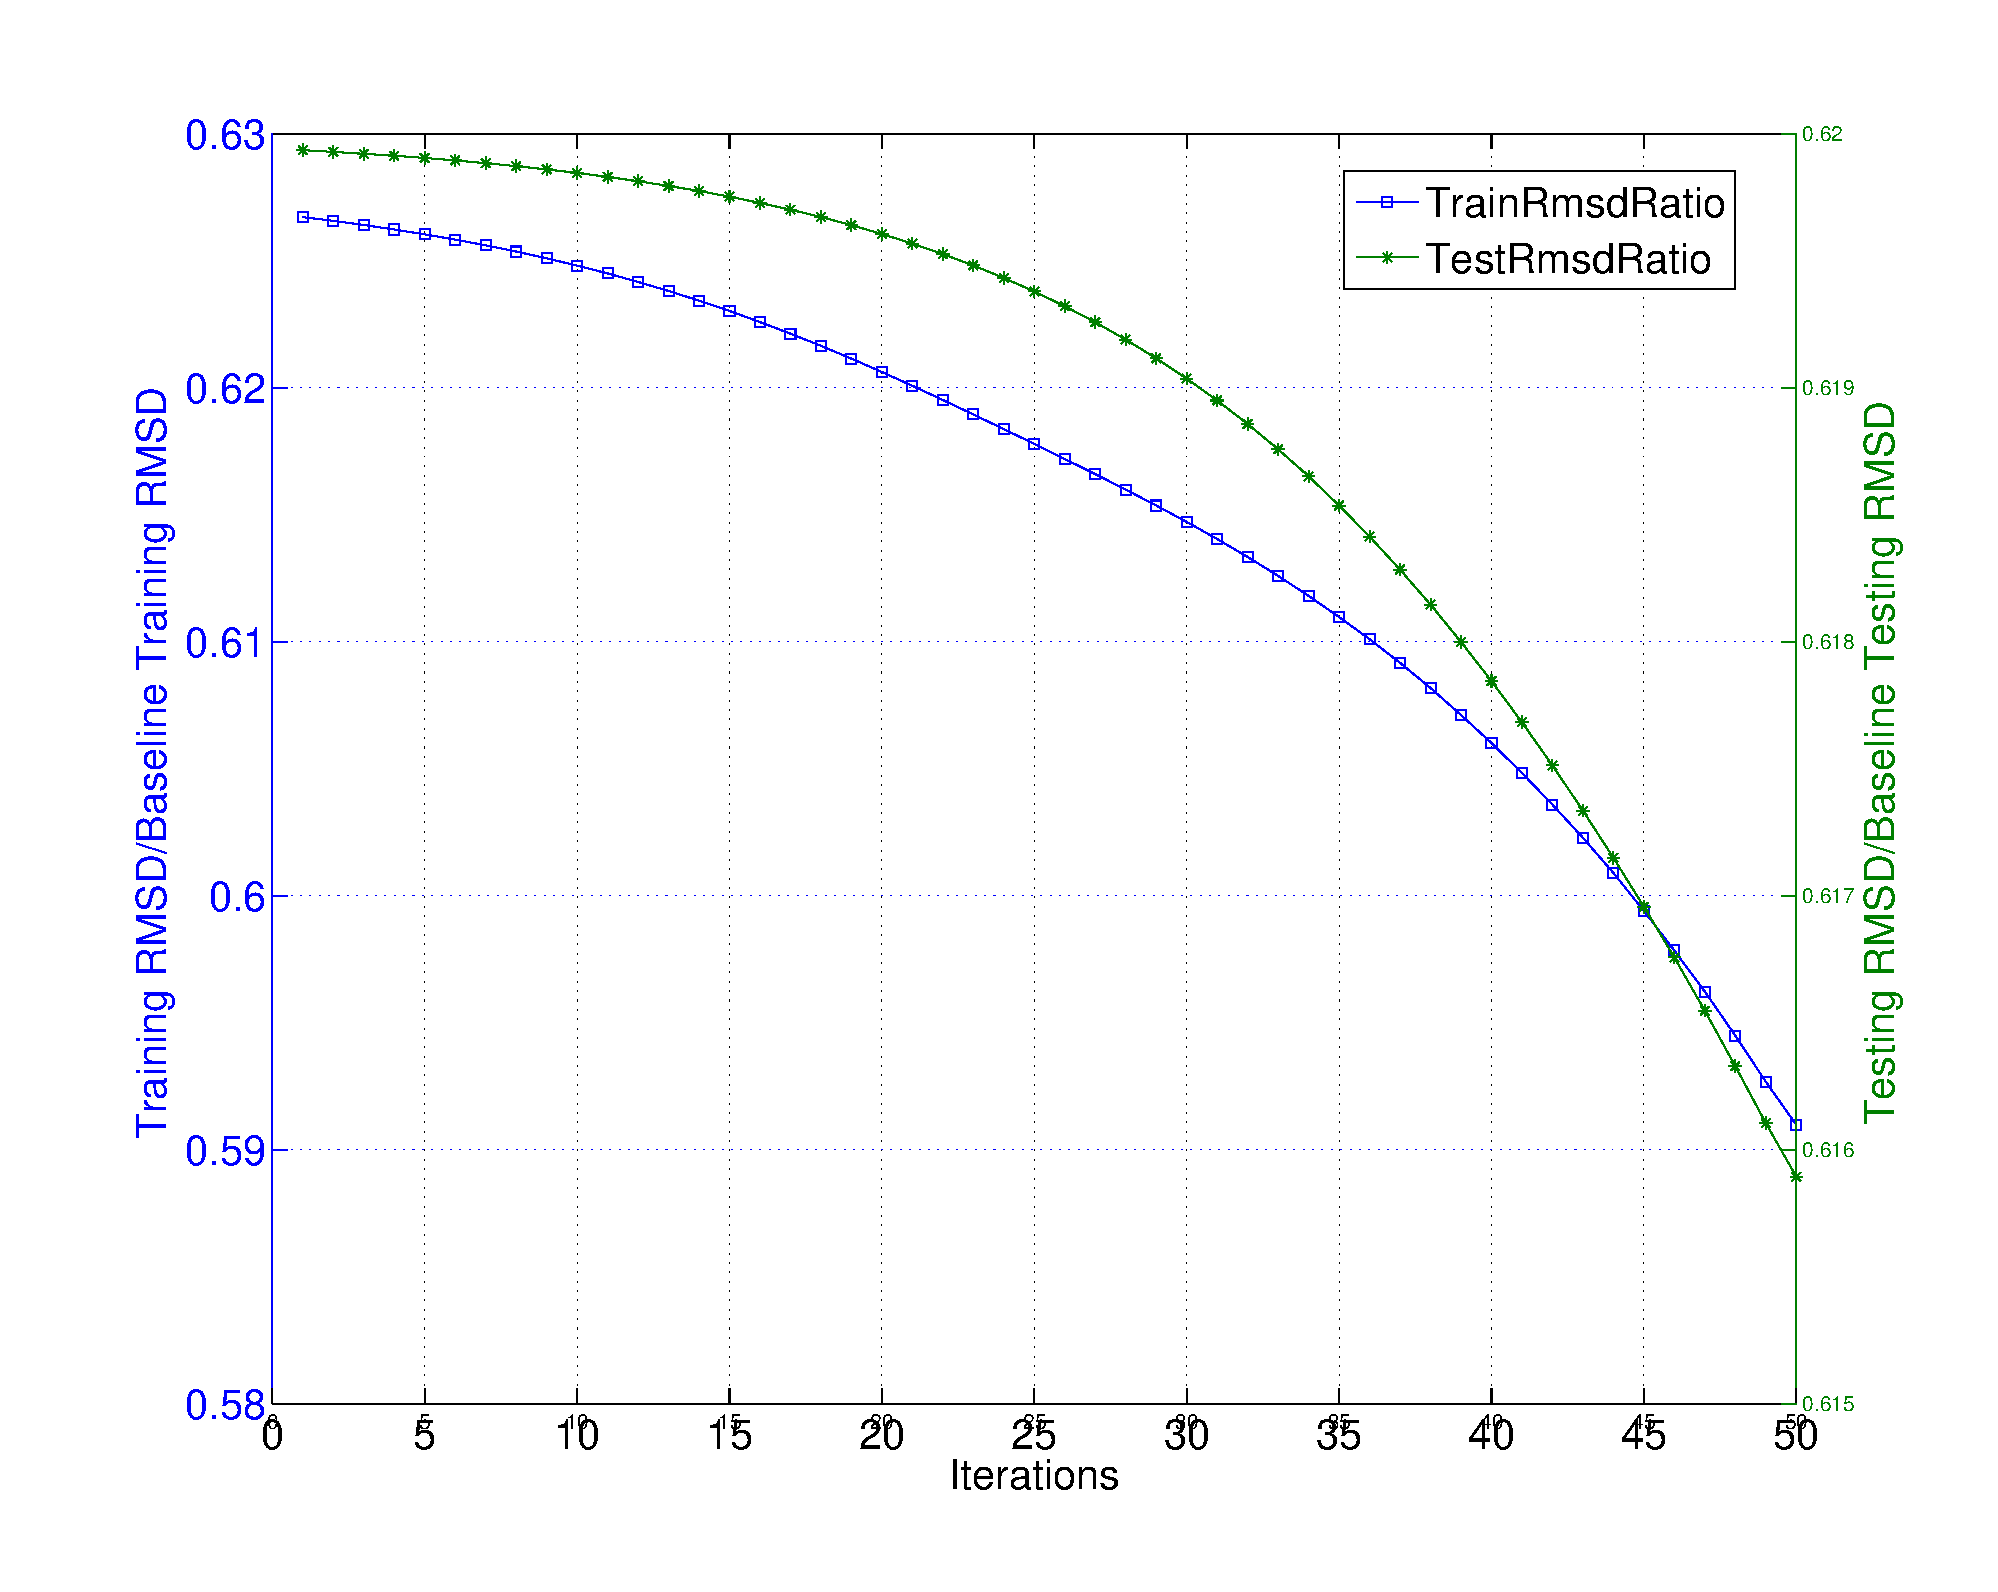
\includegraphics[width=0.42\textwidth]{figures/learning_curve_sppan_whole_relative.eps}
  \caption{{\sppan} Learning Curve on Whole Dataset}
  \label{fig:sppan_curve_whole}
\end{figure}

\subsubsection{Scalability}

Besides the experiments on $10\%$ sub sampled data set, it is worth
mentioning that the proposed {\sppan} model can also handle the whole
CTR data set on a single computer. Similar to the model evaluation
experiment on the sub-sampled data set, we separate the whole CTR data
set into a $95\%$ training set and a $5\%$ testing set through random
selection. Then, we use the $95\%$ training set to train the {\sppan}
model, and test the model on the $5\%$ testing set. The output
training RMSD ratio and testing RMSD ratio are $0.59$ and $0.62$
respectively, which shows a great improvement from the baseline
method.

We also show the learning curves of {\sppan} model in Figure
\ref{fig:sppan_curve_whole}. As we can see, both the training error
and testing error were decreasing during each training iterations
until the training stop criterion was met, which is a strong indicator
that the {\sppan} model is not over-fitted on the whole CTR data set.

\section{Related Work}
\label{sec:related}

Among the prevalence in online advertisements system, e-commerce
platform and social networks, there has been an increasing interest in
developing recommendation systems \cite{resnick1997recommender,
  ricci2011recommender} that can automatically predict the
"preference", "rating", "performance" or "interest" of a item for a
end user or a client based the history data, such as the task we
introduces in Section \ref{sec:intro}. One popular technique that has
been used in many recommendation systems is called collaborative
filtering, which is based on the intuition that if two users(or
clients) have a similar opinion on an item(or issue), they are more
likely to have similar opinions on other items(or
issues)\cite{resnick1997recommender, sarwar2001item,
  koren2011advances, ricci2011recommender}. Generally, collaborative
filtering is an approach that make use of the preference information
from many users to give prediction of the interest of one user. There
are many forms of collaborative filtering systems. For examples,
Linden et al. uses the item-to-item collaborative filtering to offer
personalized recommendations for each customer in the online
store\cite{linden2003amazon}; Cai et al. captures the interaction
between users within a social network and formulates a collaborative
filtering approach to allow high quality people to people
recommendations in social networks \cite{cai2011collaborative}; Hu et
al. implements a large scale TV recommender system with a
collaborative filtering based on prior implicit feedback that can
recommend new TV programs to their users with high accuracy
\cite{hu:2008}.

As a special type of collaborative filtering, various forms of matrix
factorization based recommendation system were used by researchers for
different recommendation tasks \cite{ZitnikZ12, lin2007projected,
  lee2001algorithms, brunet2004metagenes, parambath2013matrix,
  ricci2011recommender}. For instance, to help Flickr users more
easily engage in group activities, Zhang et al. proposes a tensor
decomposition-based Flickr group recommendation model, which is based
on CANDECOMP/PARAFAC tensor decomposition method to capture the
underlying patterns in the user-tag-group
relations\cite{zheng2010flickr}. Gu et al. introcudes a graph
regularized nonnegative matrix factorization model for general
collaborative filtering tasks, which outperform many state of the art
collaborative filtering methods on benchmark data
sets\cite{gu2010collaborative}. Other work by Baltrunas et
al. presents an context-aware matrix factorization (CAMF) method which
extends the classical Matrix Factorization approach by taking
contextual information into consideration
\cite{baltrunas2011matrix}. By applying their method on MovieAT data
set and Yahoo Webscope movie data to do movie rating prediction,
Baltrunas et al . have shown that the CAMF method can substantially
improve the rating prediction accuracy comparing to the the classical
Matrix Factorization approaches in certain circumstances in which the
relevant context information is available.

Despite there being a lot of researches of matrix factorization based
collaborative filtering methods, many algorithms still have salient
weaknesses under sparsity conditions
\cite{cacheda2011comparison}. Even though there are approaches like
multi-Domain collaborative filtering by Zhang et al. and adapting
neighborhood and matrix factorization model by Liu et al. trying to
improve the model's performance by integrating other available context
information\cite{zhang2012multi, liu2010adapting}, an extreme sparse
data set would easily make most of the matrix factorization based
models over-fitting. The SPPAN model in this present paper, however,
adjust the complexity of the model automatically according to the
sparsity of the data set, which makes it more accustomed to extreme
sparse data set.

\section{Conclusions}
\label{sec:conclusion}
In summary, the Similarity Powered Pairwise Amplifier Network
({\sppan}) model we proposed in this article shows promising results
in predicting click-through rate (CTR) in a very sparse CTR data
set. It utilizes the pairwise ratio similarity information that
embedded in the data set, and its model complexity is automatically
adjusted according to the sparsity of the data set. Comparing with
several matrix factorization based recommendation methods, our
evaluation experiment results show that this model can substantially
improving the performance of the recommendation system in extreme
sparse situations. It has also been shown that the training process of
the {\sppan} model can be easily implemented in a paralleled version
through map-reduce, which makes the model can handle even bigger data
set efficiently.

Since all evaluation experiments in this paper were performed on a
click-through rate data set, we must observe that more experimental
evaluations of the proposed {\sppan} model should be performed in the
future in order to make a more comprehensive conclusion of the
performance of the model. In fact, out next plan is to apply the
{\sppan} model on other sparse data sets from different domains so
that we could confirm if the {\it Homogeneous Amplifying Effect}
described in Section \ref{sec:model_intuition} is valid only in online
advertisement traffic data or can be generalized in other
areas. Moreover, the experiment result in the present paper only shows
the advantages of the {\sppan} model in a situation with a certain
sparsity level. A sensitivity analysis about the effect of the
sparsity on the model's performance would help us to decide when to
use {\sppan} model instead of other approaches.


% conference papers do not normally have an appendix

% use section* for acknowledgment
\ifCLASSOPTIONcompsoc
  % The Computer Society usually uses the plural form
  \section*{Acknowledgments}
\else
  % regular IEEE prefers the singular form
  \section*{Acknowledgment}
\fi

The authors would like to thank...

% trigger a \newpage just before the given reference
% number - used to balance the columns on the last page
% adjust value as needed - may need to be readjusted if
% the document is modified later
%\IEEEtriggeratref{8}
% The "triggered" command can be changed if desired:
%\IEEEtriggercmd{\enlargethispage{-5in}}

% references section

% can use a bibliography generated by BibTeX as a .bbl file
% BibTeX documentation can be easily obtained at:
% http://www.ctan.org/tex-archive/biblio/bibtex/contrib/doc/
% The IEEEtran BibTeX style support page is at:
% http://www.michaelshell.org/tex/ieeetran/bibtex/
\bibliographystyle{IEEEtran}
\bibliography{ref}
% argument is your BibTeX string definitions and bibliography database(s)
%\bibliography{IEEEabrv,../bib/paper}
%
% <OR> manually copy in the resultant .bbl file
% set second argument of \begin to the number of references
% (used to reserve space for the reference number labels box)
% \begin{thebibliography}{1}

% \bibitem{IEEEhowto:kopka}
% H.~Kopka and P.~W. Daly, \emph{A Guide to \LaTeX}, 3rd~ed.\hskip 1em plus
%   0.5em minus 0.4em\relax Harlow, England: Addison-Wesley, 1999.

% \end{thebibliography}

% that's all folks
\end{document}
